% \chapter{Piston-Driven Pneumatically-Actuated Soft Robots: Modeling and Backstepping Control}
\chapter{Backstepping Control of Piston-Driven Pneumatically-Actuated Soft Robots}
\label{chp:backstepping}

\begin{abstract}
    Actuators' dynamics have been so far mostly neglected when devising feedback controllers for continuum soft robots since the problem under the direct actuation hypothesis is already quite hard to solve. Directly considering actuation would have made the challenge too complex. However, these effects are, in practice, far from being negligible. The present chapter focuses on model-based control of piston-driven pneumatically-actuated soft robots. We propose a model of the relationship between the robot's state, the acting fluidic pressure, and the piston dynamics, which is agnostic to the chosen model for the soft system dynamics. 
    We show that backstepping is applicable even if the feedback coupling of the outer on the inner subsystem is not linear.
    Thus, we introduce a general model-based control strategy based on backstepping for soft robots actuated by fluidic drive. As an example, we derive a specialized version for a robot with piecewise constant curvature. 
\end{abstract}

\blfootnote{This chapter is based on \faFileTextO~\emph{\textbf{M. Stölzle}, C. Della Santina (2021). Piston-driven pneumatically-actuated soft robots: Modeling and backstepping control. IEEE Control Systems Letters, 6, 1837-1842.}~\cite{stolzle2021piston}.
}


%% Start the actual chapter on a new page.
\newpage

\section{Introduction}\label{sec:backstepping:introduction}
% \dropcap{C}{ontinuum} soft robots are systems entirely made of deformable materials, so to resemble the trunk of an elephant~\citep{della2020softencyclopedia}. 
% Controlling continuum soft robots is challenging because of the infinite amount of \glspl{DOF}, the multi-body dynamics, nonlinear potentials, underactuation, and the high degree of uncertainties~\citep{george2018control}. 
% Combining feedback controllers % (inherently robust to model uncertainties)
% and simplified dynamical models can help taming this complexity and achieve good experimental performance \citep{thieffry2018control, della2020model, franco2021energy}.
%
%many approaches investigated the use of the constant curvature assumption and its extensions for static and dynamic control for continuum soft robotic manipulators~\citep{della2020model}.

%
%\citep{falkenhahn2014trajectory} proposes an optimal dynamic controller for pneumatically actuated manipulators which estimates an optimal trajectory that reduces the transition time and actuator jerk. Similarly, \citep{marchese2016dynamics} describes a trajectory optimization scheme for a soft planar manipulator. Clearly, there is need to not only incorporate the actuator dynamics into the trajectory planning, but also in the actual joint control. 

% Related work
% types of fluidic actuators

%While the actuator dynamics are often negligible for tendon-driven robots, the actuator dynamics of pneumatic actuators are slower and more nonlinear~\citep{george2018control}. 

% modeling
\dropcap{A}ccurate low-dimensional models of the continuum dynamics have been thoroughly investigated in recent years~\citep{faure2012sofa, grazioso2019geometrically, sadati2021tmtdyn}, serving as the base for model-based controllers \citep{boyer2020dynamics, della2023model}. 
In comparison, researchers have devoted little or no attention to modeling the actuator dynamics, despite this being far from a negligible effect in practice, in particular for pneumatic actuation. %Consider for example pneumatic actuation \citep{x}. 
%Simplified linear models 
%To the best of the authors' knowledge, the only work explicitly dealing with this challenge is \citep{wang2017soft}, which proposes a simplified model for a soft robotic gripper.
%
% In contrast, fewer publications investigate the modeling of the kinematics and dynamics of the mapping from actuation to configuration space. \citep{wang2017soft} proposes a simplified dynamic model for soft robotic grippers by considering the  deformation in a two-dimensional plane and dividing the Fluidic Elastomer Actuator (FEA) into a sequence of $n$ line segments with constant length. Viscoelastic joints are used to connect the segments with the bending motion generated by chamber expansion modeled by a series of rotational torques acting on each joint. The Euler-Lagrangian equation is used to derive the dynamics of the system of segments.  Experiments show a almost linear relationship between applied air pressure and bending angles for some FEAs while other FEAs incorporate slight nonlinear behaviours~\citep{wang2017soft}.
%
%Fluidic drive cylinders can have certain advantages over other fluidic energy supplies such as solenoid valves as for the fact that the segment curvature is monotonically related to the cylinder displacement, there is no exchange of fluid with the environment and the fluid flow can be continuously adjusted~\citep{marchese2016design}.
%
% PID controllers
The lack of models pairs with the scarcity of model-based dynamic controllers. Existing strategies only rarely reason on the actuators' dynamics, if not through simple heuristics.
%
For example, \citep{lindenroth2016stiffness, marchese2016design, della2020model} use a combination of PID control and inversion of quasi-static linear approximations to compensate for the actuators' dynamics.
%
This strategy may present clear limitations in terms of performance and stability assessment.
%
%to relate the desired torque in configuration space $\Bar{\tau}$ to a commanded actuation sequence of solenoid valves or to the actuation of pneumatic pistons. %A cascaded control approach is applied with an inner PID loop controlling pistons, and an outer loop controlling the curvature of the arm in~\citep{marchese2014design}. 
%
% Even when PID controllers work, well %because of the mostly linear relationship between chamber pressure and robot configuration for a limited pressure range~\citep{lindenroth2016stiffness}, 
% the gains are intricate to tune, and sensitive to changes in the robot design or actuator parameters.
%
% As an alternative, \citet{gillespie2016simultaneous} propose a data-driven approach combined with an MPC controller.
% This sometimes works reasonably well as some experiments show a mostly linear relationship between chamber pressure and robot configuration for a limited pressure range~\citep{lindenroth2016stiffness}.
% 
% \citet{marchese2014design, marchese2016design} models the the dynamics of a pneumatic drive cylinder and the relationship between the change in fluid pressure inside the chambers of the arm segment and the pressure in the fluidic drive cylinder as a parameter of wall resistance and the compliance of elastomeric channels. Further, they also model the force output of an electric linear actuator to drive the fluidic cylinder dependent on the input motor voltage. This model however, is not used for control purposes and their controller relies on a cascaded control feedback algorithm with an inner PID loop running at \SI{1}{kHz} to control the position of the linear actuator and an outer loop executed at \SI{20}{Hz} to control the curvature of the arm segment by adapting the demanded piston position~\citep{marchese2014design}.

% sliding mode controller
% Sliding mode controllers based on second order lumped system dynamics have been explored to control a soft pneumatic actuator through the means of solenoid valves~\citep{skorina2015feedforward}. 
% The sliding mode controller was bench-marked against an additional feedforward term. The sliding mode controller together with the feedforward term shows the best tracking performance.

\begin{figure}[t]
  \centering
  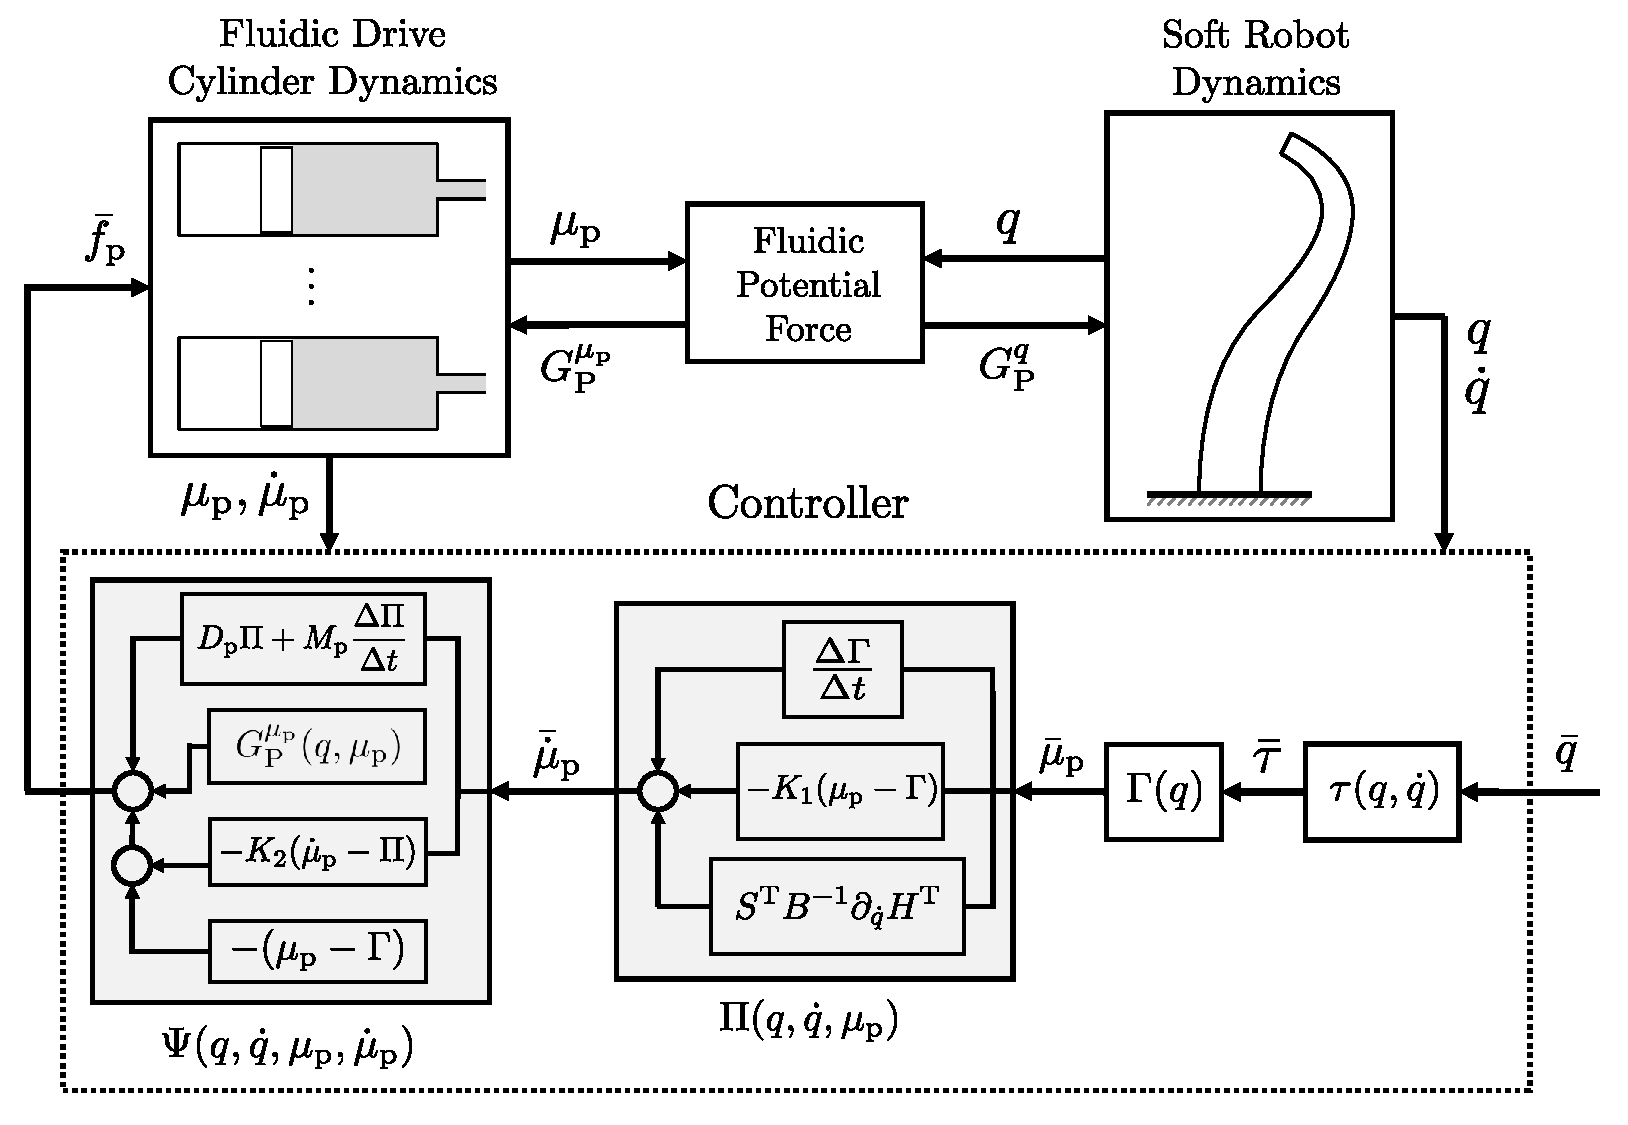
\includegraphics[width=0.9\columnwidth]{backstepping/figures/backstepping_graphics_control_scheme_v3_cropped.pdf}
  \caption{Schematic block diagram of the proposed nonlinear backstepping controller for a pneumatically-actuated soft robot. The approach considers both the fluidic drive cylinder and the soft system dynamics. It is agnostic to the chosen soft system controller in configuration-space $\tau(q,\dot{q})$.}\label{fig:backstepping:control_scheme}
\end{figure}

As model-based control of soft robots becomes a mature discipline, the need for general ways of dealing with actuators' dynamics becomes more pressing. In this chapter, we deal with this challenge by following a backstepping approach, which is an established strategy to deal with dynamical systems with a triangular structure. %We focus on piston-driven pneumatically-actuated soft robots.
%
A pneumatic model based on the ideal gas law is derived, and the pneumatic actuation system is compensated in a quasi-static fashion in \citet{falkenhahn2016dynamic}.
%
% Seminal works have dealt with underactuated robotic systems using backstepping, as non-holonomic robots in \citep{fierro1997control}, flexible joint robots in \citep{oh1999control}, a single pneumatic muscle actuator in \citep{carbonell2001nonlinear}, variable stiffness actuated robots in \citep{petit2015backstepping}.
%
% For cable-driven soft continuum robots, a dynamic model based on strain-parametrization is developed in \citep{boyer2020dynamics} and subsequently used for CT control exploiting the triangular differential structure between the torques on the robot configuration and the applied cable tensions.
% with a composite control law consisting of fast part damping the configuration dynamics around the equilibrium trajectory determined by the slow control component.
%
Recent work by \citet{wang2019parameter} uses backstepping for control of a continuum soft bending arm. Although interesting, the work is limited because it targets a linear model of a single \gls{DOF}.
Similarly, \citet{franco2021nonlinear} derive an energy-based control scheme for pneumatic manipulators while using a backstepping-based controller for comparison purposes.
% 
%{In a separate work considering the control of the \gls{BHA}, a pneumatic model based on the ideal gas law is derived and the pneumatic actuation system is controlled using a feedback-linearization controller that can compensate for the nonlinearities of the model~\citep{falkenhahn2016dynamic}.
Both pieces of work focus on pneumatic actuation with valves and thus cannot be immediately applied to systems actuated with fluidic drive cylinders.

To conclude, this chapter targets the dynamic control of piston-driven pneumatic-actuated soft robots (see, for example, Fig.~\ref{fig:backstepping:fluidic_drive_cylinder},~\ref{fig:backstepping:pcc_case_overview}). 
We provide general strategies for (i) augmenting existing dynamic models of soft robots through a description of pneumatic actuation, (ii) controlling these systems via model-based feedback. 
% Note that the application of backstepping is made not trivial by the non affine nature of the potential coupling. 
As an example, we specialize the model to planar soft robots satisfying the \gls{PCC} assumption~\citep{della2020model}, including the proposal of a kinematic model for the air volume in the chambers, and the controller for the set-point regulation of configuration. In this context, we also propose a simplified, potential coupling-aware PID-like controller. We provide simulations showing the effectiveness of both strategies.

% backstepping
% Some recent work by \citet{wang2018design, wang2019parameter} uses backstepping for control of a continuum soft bending arm with one \gls{DOF} actuated by pneumatic solenoid valves. A second-order transfer function is used to describe the dynamic behaviour from the driving pneumatic pressure to the continuum soft bending arm.
%\textcolor{red}{TODO: Explicitely describe how our approach is different}
% \citep{wang2018design} and \citep{wang2019parameter} approximate the air dynamics of a pneumatic solenoid valves and identifies the parameters using least-squares fitting. A second-order transfer function is used to describe the dynamic behaviour from the driving pneumatic pressure to the continuum soft bending arm. This dynamic model of the pressure regulator is used to control a bending actuator with one degree of freedom via backstepping to the PVM signal of the valve. Experiments show a superior trajectory tracking performance compared to a PID controller.
% Backstepping with load observation is also used to control a hydraulically controlled excavator by to compute the desired hydraulic force for motion tracking~\citep{bao2020energy}.
% Recent work analytically derives the chamber length of a soft actuator with three degrees of freedom as a function of input pressure with a Neo-Hookean deformation model only considering the kinematics of the system~\citep{xie2020design}. This model is used for inverse kinematic control of the input pressure for demanded azimuth and bending angles. Experiments to verify the analytical kinematic model show a considerable underestimation of the real bending angle.

% trajectory planning
% The full modelled dynamics of a continuum soft robot arm can also be leveraged within trajectory planning algorithms for bracing and grabbing strategies~\citep{marchese2016dynamics}. The system is broken down into three subsystems consisting of the fluidic drive cylinders, fluidic elastomer actuators and the soft manipulator with parameters identified from experimental data.
% One can further leverage the full modelled dynamics of a continuum soft robotic arm for trajectory planning algorithms such as for bracing and grabbing strategies~\citep{marchese2016dynamics}. They derive the fluidic energy stored in the system including a component lost due to resistivity of the fluid transmission line and viscous fluid friction. A cubic relationship between internal chamber volume and generalized torque on the system with a linear relationship between volume and bending angle is modelled and additionally a delay due to the impedance of the fluid transmission line introduced. The robotic arm is modelled with four fluidic drive cylinder pairs. The system is broken down into three subsystems consisting of fliudic drive cylinders, fluidic elastomer actuators mapping the cylinder displacements into generalized torques and the soft manipulator mapping the generalized torques into manipulator states. System identification techniques are used to identify the parameters of the modelled relationship between cylinder displacement and the generalized torques.

% contributions
%We state the contributions of this chapter as:
%
% To conclude, this chapter contributes to the state of the art in modeling and controlling soft robots with
% %
% \begin{itemize}
%     \item A strategy for including \textcolor{orange}{(Maxi) models of the actuation dynamics of pneumatically-driven soft robots into the control strategy. }
%     \item We propose a novel model-based, nonlinear and dynamic controller to pneumatically actuate fluidic drive cylinders in the framework of continuum soft robots. The approach is general and agnostic to the specific control strategy used for the soft manipulator.
%     \item We derive an analytical model for the volume in the pneumatic chambers of a continuum soft robot under \gls{PCC} assumption as a function of the configuration and subsequently develop a specialized controller for the \gls{PCC}-case.
% \end{itemize}
\section{Dynamic Model}\label{sec:backstepping:dynamic_model}

We consider the robot made by a sequence of $n_{\mathrm{S}} \in \mathbb{N}_+$ segments. Each segment is described with $n_{\mathrm{D}} \in \mathbb{N}_+$ configuration variables by using one of the many modeling techniques being developed in the state-of-the-art~\citep {faure2012sofa, grazioso2019geometrically, sadati2021tmtdyn, boyer2020dynamics}.
%
We denote with $n_{\mathrm{q}} = n_{\mathrm{S}} n_{\mathrm{D}}  \in \mathbb{N}_+$ the total number of configuration variables, which also represents the approximated \glspl{DOF} of the soft arm.
%
Although we show planar kinematic relations for the \gls{PCC}-case in Figure~\ref{fig:backstepping:pcc_case_overview} as an example, the dynamic model derived in this section is agnostic to the chosen kinematic approximation.
%

All kinematic modeling techniques produce multi-body dynamics of the unactuated soft robot as follows~\citep{della2023model}
%
\begin{equation}
	M(q)\ddot{q} + C(q,\dot{q}) \dot{q} + G(q) + K(q) + D(q, \dot{q}) = 0,
\end{equation}
%
where $q \in \mathbb{R}^{n_{\mathrm{q}}}$ describes the configuration of the robot in generalized coordinates, $M(q) \in \mathbb{R}^{n_{\mathrm{q}} \times n_{\mathrm{q}}}$ the inertial matrix, $C(q,\dot{q}) \in \mathbb{R}^{n_{\mathrm{q}} \times n_{\mathrm{q}}}$ contains the Coriolis and Centrifugal forces and $G(q) \in \mathbb{R}^{n_{\mathrm{q}}}$ compensates for the gravitational effects. The elastic (restoring) forces are captured in the matrix $K \in \mathbb{R}^{n_{\mathrm{q}}}$ and the natural damping is represented by $D(q,\dot{q}) \in \mathbb{R}^{n_{\mathrm{q}}}$.

%
Each segment is actuated through a set of $n_{\mathrm{C}}$ dedicated chambers.
%
Adapting the pressure in a chamber will lead to a different chamber volume, ultimately resulting in a changed configuration of the segment.
%
Each chamber is connected to a dedicated piston, as shown in Figure~\ref{fig:backstepping:pcc_case_overview}. If more than one chamber is connected to the same piston, it can be considered to be the same chamber for the sake of this chapter.
%
These hypotheses are not paramount, but they are instrumental in making the notation easier.
%
Accordingly, the total number of pistons is described with $n_{\mu_\mathrm{p}} = n_{\mathrm{S}} n_{\mathrm{C}}$.
%
Please note that if $n_\mathrm{C} = n_\mathrm{D}$, the model of the soft robot is fully-actuated, if $n_\mathrm{C} > n_\mathrm{D}$ it is over-actuated, and with $n_\mathrm{C} < n_\mathrm{D}$ under-actuated respectively.
%
The dynamics of the piston, when not interacting with the fluid, can be easily written as being
%
\begin{equation}
M_\mathrm{p} \ddot{\mu}_\mathrm{p} + D_\mathrm{p} \dot{\mu}_\mathrm{p} + G_{\mathrm{P}}^{\mu_p} = f_\mathrm{p},
\end{equation}
%
where $\mu_\mathrm{p} \in \mathbb{R}^{n_{\mu_\mathrm{p}}}$ denoting the displacement of every piston from the zero-volume configuration, $M_\mathrm{p} \in \mathbb{R}^{n_{\mu_\mathrm{p}} \times n_{\mu_\mathrm{p}}}$ the mass matrix of the piston system, $G_{\mathrm{P}}^{\mu_p} \in \mathbb{R}^{n_{\mu_\mathrm{p}}}$ describing the conservative force caused by the compressed fluid acting on the pistons, and $D_\mathrm{p} \in \mathbb{R}^{n_{\mu_\mathrm{p}} \times n_{\mu_\mathrm{p}}}$ the damping matrix of the piston system. 
As the piston system is fixed to the ground and connected via tubing to the robot chambers, note that the gravity force here is constant, so w.l.o.g., we consider it to be zero (or alternatively as being compensated by a constant offset in $f_\mathrm{p}$).

\begin{figure}[ht]
  \centering
  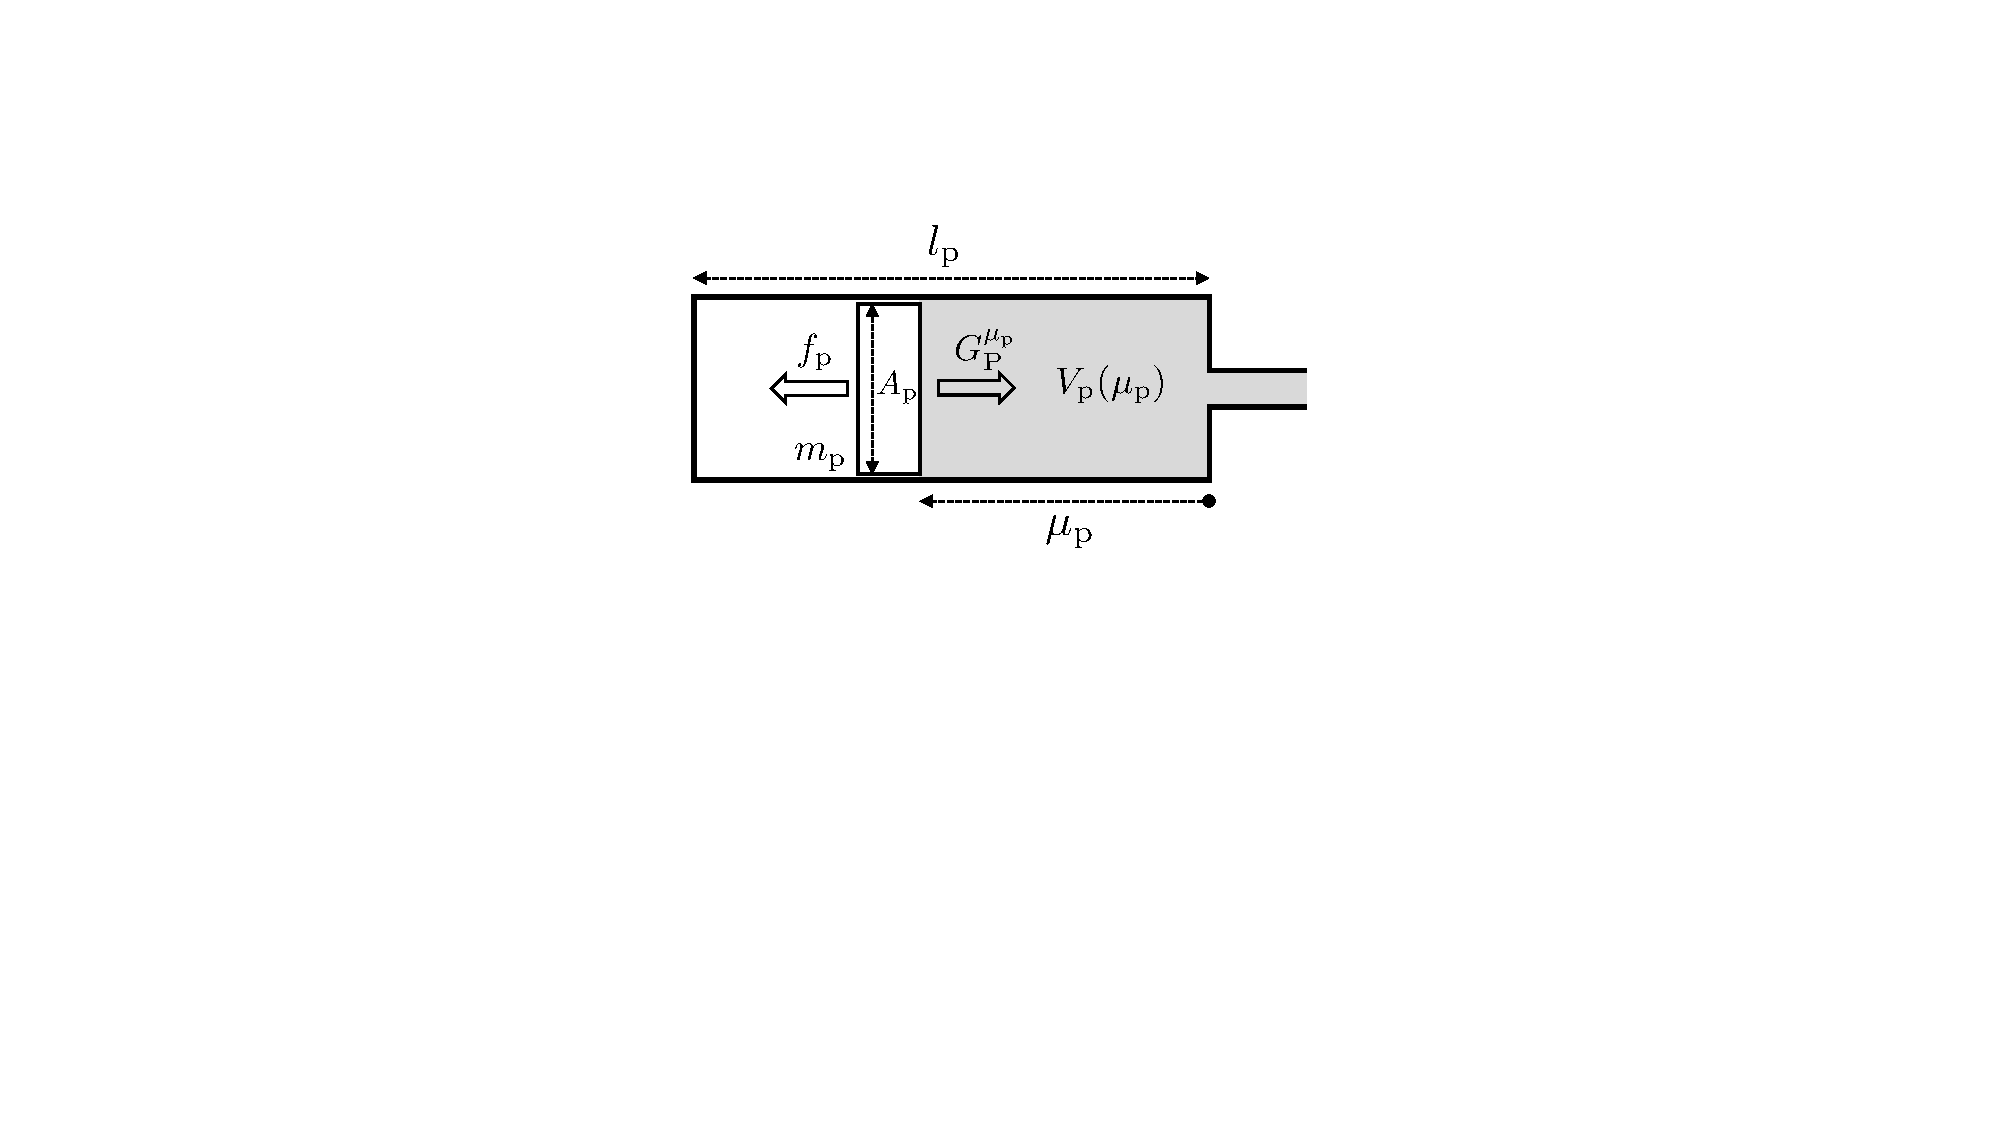
\includegraphics[width=0.5\columnwidth]{backstepping/figures/backstepping_graphics_fluidic_drive_cylinder_v4.pdf}
  \caption{Fluidic drive cylinder parameters for a piston of mass $m_\mathrm{p}$, length $l_\mathrm{p}$ and cross-sectional area $A_\mathrm{p}$: $f_\mathrm{p}$ describes the actuation force while $G_\mathrm{P}^{\mu_\mathrm{p}}$ is the conservative force applied by the compressed fluid on the cylinder. $\mu_\mathrm{p}$ represents the actuators' state variable. These pneumatic pistons could be, for example, actuated by current-controlled DC motors or linear electric actuators~\citep{marchese2014design}.}\label{fig:backstepping:fluidic_drive_cylinder}
\end{figure}

\begin{figure}[ht]
  \centering
  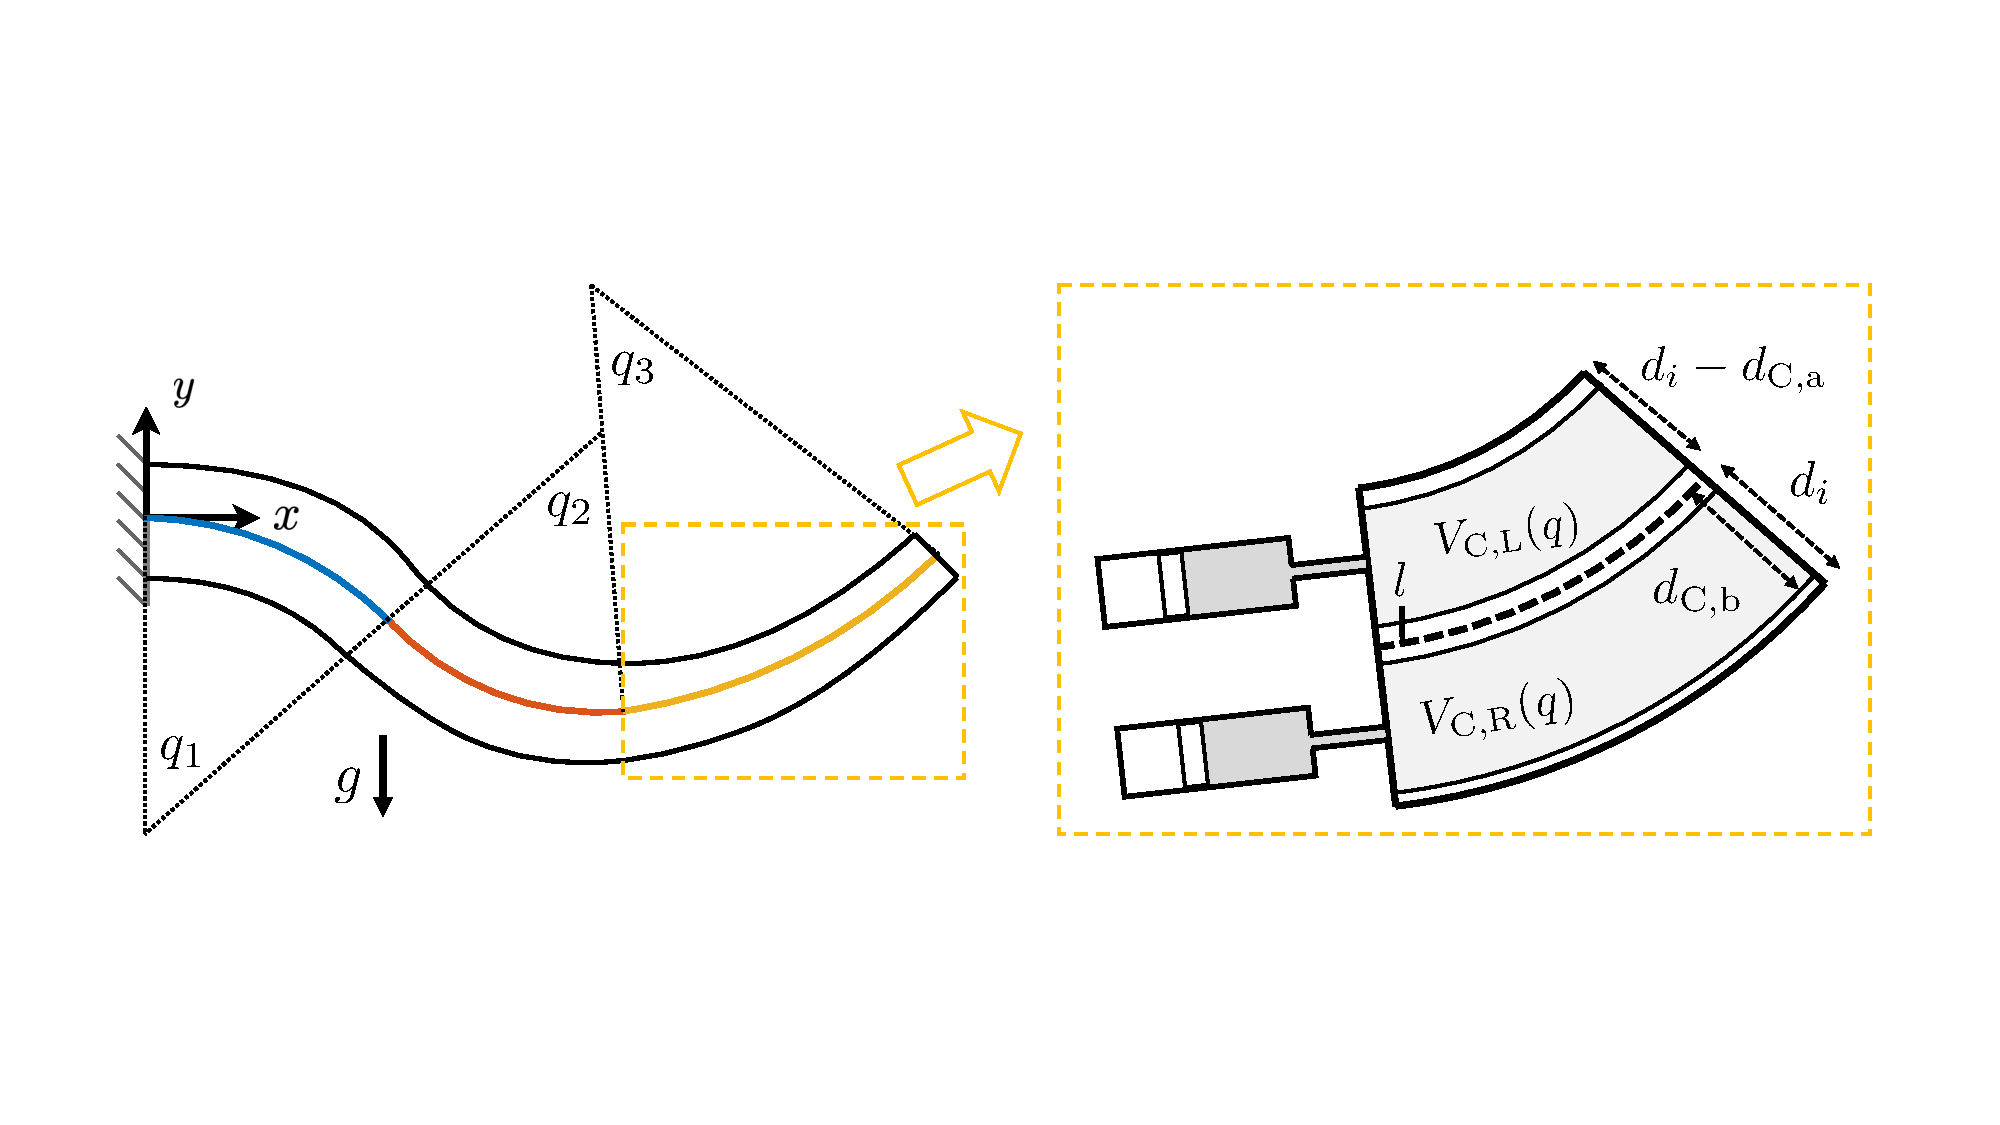
\includegraphics[width=0.9\columnwidth]{backstepping/figures/backstepping_graphics_pcc_case_overview_v4_cropped.pdf}
  \caption{Shape regulation under \gls{PCC} approximation - \textbf{Left:} A planar soft robot consisting of three segments, each modeled to have constant curvature \textbf{Right:} Model parameters for fluidic volume in soft segment chambers. Each chamber is actuated independently by a fluidic drive cylinder connected through tubing.}\label{fig:backstepping:pcc_case_overview}
\end{figure}


In the first approximation, we model the compressible fluid (typically air) as an ideal gas. Furthermore, we consider the process to be isothermal, and no fluid exchange with the external world is happening. We neglect the volume of fluid in any tubes connecting the pistons with the chambers.
%
The overall volume of the fluid can be evaluated as %the sum of the chamber volume $V_{\mathrm{q},i}(q)$
%
%\begin{equation}
%	V_i(q_i,l_{c(i)}) = \sum_{j \in c(i)} V_{\mathrm{q},j}(q_i) + A_{c(i)}^{\top}  l_{c(i)}, 
%\end{equation}
%%
%where $c:\mathbb{N} \rightarrow \mathbb{N}^{n_{\mathrm{C}}}$ is the function returning the indexes of chambers actuating the $i\--$th segment.
\begin{equation}
V(q,\mu_\mathrm{p}) = V_{\mathrm{C}}(q) + V_{\mathrm{p}}(\mu_{\mathrm{p}}) = V_{\mathrm{C}}(q) + A_{\mathrm{p}} \mu_{\mathrm{p}}, 
\end{equation}
%
where $V(q,\mu_\mathrm{p}) \in \mathbb{R}^{n_{\mu_\mathrm{p}}}$ describes the total volume of fluid stored in the system, $V_{\mathrm{C}}(q) \in \mathbb{R}^{n_{\mu_\mathrm{p}}}$ the volume of fluid in each chamber and $V_{\mathrm{p}}(q) \in \mathbb{R}^{n_{\mathrm{S}} n_{\mathrm{p}}}$ the volume in the piston with $A_{\mathrm{p}} \in \mathbb{R}^{n_{\mu_\mathrm{p}}}$ the cross-sectional area of every piston.
%
% The function $V_{\mathrm{C}}(q)$ can be either analytically derived or learned off\--line from data. 
% move the following potentially to future work
% A possibility that we do not investigate here for the sake of space is to parametrize $V_{\mathrm{C}}(q)$  w.r.t. a set of unknown quantities $\pi$, and then learn $\pi$ on\--line through adaptive control.
%
We will present an example of analytical derivation of $V_{\mathrm{C}}(q)$ in Section~\ref{sub:backstepping:pcc_model}.
For now, we consider it known.

The total energy stored in the system due to fluid compression is
%
\begin{equation}
\begin{split}
	\mathcal{U}_\mathrm{fluid}(q,\mu_\mathrm{p}) =& \: \sum_{j = 1}^{n_{\mu_\mathrm{p}}} \int_{V_{j,0}}^{V_j(q_i,\mu_{\mathrm{p},j})} -\left ( p_j(\nu) - p_\mathrm{atm} \right ) \mathrm{d} \nu\\
	% = \sum_{j = 1}^{n_{\mu_\mathrm{p}}} \alpha_{\mathrm{air},j} \int_{V_{j,0}}^{V_j(q,\mu_\mathrm{p})} -\left ( \frac{1}{\nu} - \frac{1}{V_{j,0}} \right ) \mathrm{d} \nu\\
	=&\: \sum_{j=1}^{n_{\mu_\mathrm{p}}} - \alpha_{\mathrm{air},j} \left ( \ln  \frac{V_j(q_i, \mu_{\mathrm{p},j})}{V_{j,0}} - \frac{V_j(q_i, \mu_{\mathrm{p},j})}{V_{j,0}} + 1 \right ),
\end{split}
\end{equation}
%
where $V_j(q_i, \mu_{\mathrm{p},j}) = \frac{\alpha_{\mathrm{air},j}}{p_j(q_i, \mu_{\mathrm{p},j})}$ represents the total fluidic volume in the system of chamber and piston $j$ in segment $i$. We assume that this fluid system is filled with air at atmospheric pressure $p_\mathrm{atm}$ with an initial volume of $V_{j,0} = V_j(0, l_\mathrm{p})$ (e.g., straight robot configuration and with fully extended pistons). 
This lets us find an expression for $\alpha_{\mathrm{air}}$:
\begin{equation}
    \alpha_{\mathrm{air},j} = n_j R T = p_\mathrm{atm} V_{j,0} = p_{j}(q,\mu_\mathrm{p}) V_{j}(q,\mu_\mathrm{p}).
\end{equation}
%
% More complex pressure\--volume relationships involving not constant $n_j$ will be the topic of future investigations.

The force exerted on the $i$th segment of the robot by the fluid is 
%
%\begin{equation}
%		G_{\mathrm{P},j}^{\mathrm{q}}(q,l) = \partial_{q_j} E =  \sum_{i \in c(j)} \alpha_i \frac{\partial_{q_j}V_{\mathrm{q},i}}{V_{\mathrm{q},i}(q) + A_i l_i}, 
%\end{equation}
\begin{equation}\label{eq:backstepping:GPq}
\begin{split}
    G_{\mathrm{P},i}^{\mathrm{q}}(q_i,\mu_{\mathrm{p},j}) &= \partial_{q_i} \mathcal{U}_\mathrm{fluid}(q,\mu_\mathrm{p}) = -\partial_{q_i} V_{C,j} \left ( p_{j}(q_i, \mu_{\mathrm{p},j}) - p_\mathrm{atm} \right ), 
\end{split}
\end{equation}
Similarly, the force applied on the $j$th piston by the fluid is
%
\begin{equation}\label{eq:backstepping:GPmu}
\begin{split}
    G_{\mathrm{P},j}^{\mu_\mathrm{p}}(q_i,\mu_{\mathrm{p},j}) &= \partial_{\mu_{\mathrm{p},j}} \mathcal{U}_\mathrm{fluid}(q,\mu_\mathrm{p}) = - A_{\mathrm{p},j} \left ( p_{j}(q_i, \mu_{\mathrm{p},j}) - p_\mathrm{atm} \right ), 
\end{split}
\end{equation}
%
The overall dynamic model is
%
\begin{equation}\label{eq:backstepping:complete_dyn} %
\begin{split}
	M(q)\ddot{q} \!+\! C(q,\dot{q})\dot{q} \!+\! G(q) \!+\! K(q) \!+\! D(q,\dot{q}) \!+\! G_{\mathrm{P}}^{\mathrm{q}}(q,\mu_\mathrm{p}) &= 0, \\
	M_\mathrm{p} \ddot{\mu}_\mathrm{p} + D_\mathrm{p} \dot{\mu}_\mathrm{p} + G_{\mathrm{P}}^{\mu_\mathrm{p}}(q,\mu_\mathrm{p}) &= f_\mathrm{p}, \; 
\end{split}
\end{equation}
which is always underactuated.
%
Note that this structure is similar to classic flexible joint robots under Spong's approximation \citep{della2021flexible} due to the fact that the fluidic drive cylinders are fixed to the ground. Two of the major differences making the control problem harder are that that $n_{\mu_\mathrm{p}} \neq n_{\mathrm{q}}$, and that $G_{\mathrm{P}}^{\mathrm{q}}$ and $G_{\mathrm{P}}^{\mu_\mathrm{p}}$ are not linear.
The latter renders the feedback coupling of the outer on the inner subsystems non-affine.
%
In the rest of the chapter, we will use the following definitions to simplify the notation
%
\begin{small}
\begin{equation}\label{eq:backstepping:gf}
\begin{split}
	f(q,\dot{q}) &= - B^{-1}(q)\left(C(q,\dot{q})\dot{q} + G(q) + K(q) + D(q, \dot{q}) \right), \\
	g(q,\mu_\mathrm{p}) &= - B^{-1}(q) \left ( G_{\mathrm{P}}^{\mathrm{q}}(q,\mu_\mathrm{p}) \right ).
\end{split}
\end{equation}
\end{small}
\section{Backstepping Control}\label{sec:backstepping:backstepping_proof}

This section discusses the main contribution of this chapter, a backstepping-based approach to generalize controllers $\Gamma(q,\dot{q})$ designed in the directly actuated case, to systems that can be modeled through \eqref{eq:backstepping:complete_dyn}.
We suppose that we have access to $\Gamma(q, \dot{q})$ controlling the piston position $\mu_\mathrm{p}$. Next, we perform backstepping twice to the controllers of the piston velocity $\dot{\mu}_\mathrm{p}$ and the piston actuation force $f_\mathrm{p}$ and prove the stability of each controller with Lyapunov arguments.
The derived model-based control approach assumes that all model parameters are known, and all states are measurable (namely the configuration $q$, its time derivative $\dot{q}$, the piston position $\mu_\mathrm{p}$ and the piston velocity $\dot{\mu}_\mathrm{p}$), and that there are no disturbances or model uncertainties. 
We first introduce a Lemma, which will be instrumental to the proof of the main theorem. It allows us to relate an offset in the actuation space to a change in acceleration in the configuration space that is proportional to the offset.
%
\begin{lemma}\label{lemma:f_g_S}%{\color{red} I have the feeling that words are missing here}
The input field defined in \eqref{eq:backstepping:gf} verifies
%
\begin{equation*}
    g(q,\mu_{\mathrm{p},\mathrm{a}}) - g(q,\mu_{\mathrm{p},\mathrm{b}}) \!=\!  -B^{-1}\!(q)S(q,\mu_{\mathrm{p},\mathrm{a}},\mu_{\mathrm{p},\mathrm{b}})(\mu_{\mathrm{p},\mathrm{a}} \!- \mu_{\mathrm{p},\mathrm{b}}),    
\end{equation*}
%
$\forall \mu_{\mathrm{p},\mathrm{a}},\mu_{\mathrm{p},\mathrm{b}} \in \mathbb{R}^{n_{\mu_\mathrm{p}}}$ and $q \in \mathbb{R}^{n_{\mathrm{q}}}$
	with $S \in \mathbb{R}^{n_{\mathrm{q}} \times n_{\mu_\mathrm{p}}} $ defined via
	%
	\begin{equation*}
	    S_{ij} = \frac{ A_{\mathrm{p},j} \alpha_{\mathrm{air},j} \partial_{q_i}V_{\mathrm{C},j}}{(V_{\mathrm{C},j}(q_i) + A_{\mathrm{p},j} \mu_{\mathrm{p},\mathrm{a},j})(V_{\mathrm{C},j}(q_i) + A_{\mathrm{p},j} \mu_{\mathrm{p},\mathrm{b},j})}.
	\end{equation*}
\end{lemma}
%
\begin{proof}
	We express the left term of the equality using \eqref{eq:backstepping:gf}
	%
	\begin{equation*}%\footnotesize
	\begin{split}
	g(q,\mu_{\mathrm{p},\mathrm{a}}) - g(q,\mu_{\mathrm{p},\mathrm{b}}) 
	=-B^{-1}(q) (G_{\mathrm{P}}^{\mathrm{q}}(q,\mu_{\mathrm{p},\mathrm{a}}) - G_{\mathrm{P}}^{\mathrm{q}}(q,\mu_{\mathrm{p},\mathrm{b}})),
	\end{split}
	\end{equation*}
	%
	where we recognize the term $B^{-1}(q)$ appearing in the Lemma. The term between brackets can be adjusted by using \eqref{eq:backstepping:GPq}
	%
	\begin{equation}
	\begin{split}
		G_{\mathrm{P},i}^{\mathrm{q}}(q,\mu_{\mathrm{p},\mathrm{a}}) - G_{\mathrm{P},i}^{\mathrm{q}}(q,\mu_{\mathrm{p},\mathrm{b}}) = &-\left(\sum_{j = 1}^{n_{\mu_\mathrm{p}}}  \frac{\alpha_{\mathrm{air},j} \partial_{q_i}V_{\mathrm{C},j}}{V_{\mathrm{C},j}(q_i) + A_{\mathrm{p},j} \mu_{\mathrm{p},\mathrm{a},j}} \!-\! \sum_{j = 1}^{n_{\mu_\mathrm{p}}}  \frac{\alpha_{\mathrm{air},j} \partial_{q_i}V_{\mathrm{C},j}}{V_{\mathrm{C},j}(q_i) + A_{\mathrm{p},j} \mu_{\mathrm{p},\mathrm{b},j}}\right),  \\
	= &\sum_{j = 1}^{n_{\mu_\mathrm{p}}} \frac{A_{\mathrm{p},j} \alpha_{\mathrm{air},j} \partial_{q_i}V_{\mathrm{C},j} \, (\mu_{\mathrm{p},\mathrm{a},j} - \mu_{\mathrm{p},\mathrm{b},j})}{(V_{\mathrm{C},j}(q_i) + A_{\mathrm{p},j} \mu_{\mathrm{p},\mathrm{a},j})(V_{\mathrm{C},j}(q_i) + A_{\mathrm{p},j} \mu_{\mathrm{p},\mathrm{b},j})},\\
        = &\sum_{j = 1}^{n_{\mu_\mathrm{p}}} S_{ij} \, (\mu_{\mathrm{p},\mathrm{a},j} - \mu_{\mathrm{p},\mathrm{b},j}) = S \, (\mu_{\mathrm{p},\mathrm{a}} - \mu_{\mathrm{p},\mathrm{b}}).
	\end{split}
	\end{equation}
	%
	The Lemma follows by simple factorization of the latter term.
\end{proof}

Thus, even if the robot side of the dynamics \eqref{eq:backstepping:complete_dyn} is not affine in control when taking $\mu_\mathrm{p}$ as input, still Lemma \ref{lemma:f_g_S} provides some structure that we leverage in the next theorem.
%
% Assuming access to a soft robot controller $\tau(q,\dot{q})$ that regulates the soft robot, neglecting actuator dynamics, to the setpoint $\bar{q}$,
% Theorem~\ref{theorem:backstepping:backstepping_controller} proposes, based on the backstepping procedure, a fluidic piston force controller $f_\mathrm{p} = \Psi(q,\dot{q},\mu_\mathrm{p}, \dot{\mu}_\mathrm{p})$ which is proven to let the closed-loop system converge to the setpoint - specifically the desired soft robot configuration $\bar{q}$ and the corresponding steady-state piston position $\bar{\mu}_\mathrm{p} = \Gamma(q)$. 
% As visualized in Fig.~\ref{fig:backstepping:control_scheme}, $\Gamma(q)$ maps positions from the configuration to the actuation space, the controller $\bar{\dot{\mu}}_\mathrm{p} = \Pi(q,\dot{q},\mu_\mathrm{p})$ provides piston velocity references, which are subsequently mapped into piston force commands by $\Psi(q,\dot{q},\mu_\mathrm{p}, \dot{\mu}_\mathrm{p})$.
% $K_1 \succ 0 \in \mathbb{R}^{n_{\mu_\mathrm{p}} \times n_{\mu_\mathrm{p}}}$ is a proportional feedback gain on the error $(\mu_\mathrm{p} - \bar{\mu}_\mathrm{p})$ between actual and desired piston positions and $K_2 \succ 0 \in \mathbb{R}^{n_{\mu_\mathrm{p}} \times n_{\mu_\mathrm{p}}}$ is a proportional feedback gain on the error $(\dot{\mu}_\mathrm{p} - \bar{\dot{\mu}}_\mathrm{p})$ between actual and desired piston velocities.
Assuming a soft robot controller $\tau(q,\dot{q})$ that regulates the soft robot to the setpoint $\bar{q}$ while neglecting actuator dynamics, Theorem~\ref{theorem:backstepping:backstepping_controller} introduces—via the backstepping procedure—a fluidic piston force controller $f_\mathrm{p} = \Psi(q,\dot{q},\mu_\mathrm{p}, \dot{\mu}_\mathrm{p})$ that ensures the closed-loop system converges to the setpoint. In particular, the system reaches the desired soft robot configuration $\bar{q}$ along with the corresponding steady-state piston position $\bar{\mu}_\mathrm{p} = \Gamma(q)$. As depicted in Fig.~\ref{fig:backstepping:control_scheme}, the function $\Gamma(q)$ maps positions from the configuration space to the actuation space, while the controller $\bar{\dot{\mu}}_\mathrm{p} = \Pi(q,\dot{q},\mu_\mathrm{p})$ supplies piston velocity references that are then converted into piston force commands by $\Psi(q,\dot{q},\mu_\mathrm{p}, \dot{\mu}_\mathrm{p})$. Here, $K_1 \succ 0 \in \mathbb{R}^{n_{\mu_\mathrm{p}} \times n_{\mu_\mathrm{p}}}$ is a proportional feedback gain applied to the error $(\mu_\mathrm{p} - \bar{\mu}_\mathrm{p})$ between actual and desired piston positions, and $K_2 \succ 0 \in \mathbb{R}^{n_{\mu_\mathrm{p}} \times n_{\mu_\mathrm{p}}}$ is a proportional feedback gain on the error $(\dot{\mu}_\mathrm{p} - \bar{\dot{\mu}}_\mathrm{p})$ between actual and desired piston velocities.

\begin{theorem}\label{theorem:backstepping:backstepping_controller}
	Suppose that a $\Gamma(q,\dot{q})$ exists s.t. the reduced system
	%
	\begin{equation}\label{eq:backstepping:reduced_sys}
		\ddot{q} = f(q,\dot{q}) + g(q,\Gamma(q,\dot{q}))
	\end{equation}
	%
	converges to a desired trajectory $\bar{q}(t)$, $\forall (q(0),\dot{q}(0)) \in \mathbb{R}^{2 n_{\mathrm{q}}}$. Suppose that the convergence is proven by Lyapunov arguments through the function $H(q,\dot{q})$. Then the closed loop of the full system \eqref{eq:backstepping:complete_dyn} and the controller
	%
%	\begin{equation}
%		\begin{split}
%%			\tau &= G_{\mathrm{P}}^{\mathrm{l}} + J  \ddot{\Gamma} + (JK_1 + K_2) (\dot{l} - \dot{\Gamma}) + (K_2 K_1 - I) (l - \Gamma)\\
%%			&- J\frac{\mathrm{d}}{\mathrm{d} t}\left(M^{\top}(q,l,\Gamma)B^{-\top}(q)\partial_{\dot{q}} H^{\top}\right) \\
%%			&- K_2 M^{\top}(q,l,\Gamma)B^{-\top}(q)\partial_{\dot{q}} H^{\top}) \\
%			\tau &= G_{\mathrm{P}}^{\mathrm{l}} + J \ddot{\Gamma} + (J + I) (\dot{l} - \dot{\Gamma})  \\
%			&- \frac{\mathrm{d}}{\mathrm{d} t}\left(M^{\top}(q,l,\Gamma)B^{-\top}(q)\partial_{\dot{q}} H^{\top}\right) \\
%			&- M^{\top}(q,l,\Gamma)B^{-\top}(q)\partial_{\dot{q}} H^{\top}
%		\end{split}
%	\end{equation}
	\begin{equation}\label{eq:backstepping:pi_psi}
		\begin{split}
			f_\mathrm{p} &= \Psi = G_{\mathrm{P}}^{\mu_\mathrm{p}} + D_\mathrm{p} \Pi + M_\mathrm{p} \dot{\Pi} - K_2 (\dot{\mu}_\mathrm{p} - \Pi) - (\mu_\mathrm{p} - \Gamma),\\
			\Pi &= \dot{\Gamma} - K_1 (\mu_\mathrm{p} - \Gamma) 
			+ S^{\top}(q,\mu_\mathrm{p},\Gamma)B^{-1}(q)\partial_{\dot{q}} H^{\top},
		\end{split}
	\end{equation}
	%
	with $K_1,K_2 \succ 0$, is such that $q \rightarrow \bar{q}$ and $\mu_\mathrm{p} \rightarrow \Gamma(\bar q,\dot{\bar q})$, $\forall (\mu_\mathrm{p}(0),\dot{\mu}_\mathrm{p}(0)) \in \mathbb{R}^{2n_{\mu_\mathrm{p}}}$, and $\forall (q(0),\dot{q}(0)) \in \mathbb{R}^{2 n_{\mathrm{q}}}$.
\end{theorem}
\begin{proof}
	
	We first consider the problem of deriving a controller under the assumption that the velocity of the piston $v_\mathrm{p}$ is set by a controller. This serves as a first step toward the general solution of the problem. System \eqref{eq:backstepping:complete_dyn} is thus reduced into
	%
	\begin{equation}\label{eq:backstepping:intermediate}
	\begin{split}
	M(q)\ddot{q} \! + \! C(q,\dot{q})\dot{q} \! + \! G(q) \! + \! K(q) \! + \! D(q,\dot{q}) \! + \! G_{\mathrm{P}}^{\mathrm{q}}(q,\mu_\mathrm{p}) &= 0, \\
	\dot{\mu}_\mathrm{p} &= v_\mathrm{p}. 
	\end{split}
	\end{equation}
	%
	We introduce the following control Lyapunov candidate
	%
	\begin{equation}
		W(q,\dot{q},\mu_\mathrm{p}) = H(q,\dot{q}) + \frac{1}{2}(\mu_\mathrm{p} - \Gamma)^{\top}(\mu_\mathrm{p} - \Gamma)\;,
	\end{equation}
	%
	which can thus be differentiated obtaining
	%
	\begin{equation}
		\begin{split}
			\dot{W}(q,\dot{q},\mu_\mathrm{p}) =& \: \dot{H} + (\mu_\mathrm{p} - \Gamma)^{\top}(v_\mathrm{p} - \dot\Gamma)\\
			=&  \: \partial_{q} H \dot{q} + \partial_{\dot{q}} H (f(q,\dot{q}) + g(q,\mu_\mathrm{p})) + (\mu_\mathrm{p} - \Gamma)^{\top}(v_\mathrm{p} - \dot\Gamma) \\
			=& \: \partial_{q} H \dot{q} + \partial_{\dot{q}} H (f(q,\dot{q}) + g(q,\Gamma(q,\dot{q}))) \\
			& \: + \partial_{\dot{q}} H (g(q,\mu_\mathrm{p}) - g(q,\Gamma(q,\dot{q}))) + (\mu_\mathrm{p} - \Gamma)^{\top} (v_\mathrm{p} - \dot\Gamma)\;,
		\end{split}
	\end{equation}
	%
	where we first used the chain rule on $\dot{H}$ and then we added and subtracted $\partial_{\dot{q}} H g(q,\Gamma(q,\dot{q}))$.
	%
	We now propose the controller $v_\mathrm{p} = \Pi(q,\dot{q},\mu_\mathrm{p})$ for stabilizing this system, with
	%
	\begin{equation*}
		\begin{split}
			\Pi(q,\dot{q},\mu_\mathrm{p}) &= \dot{\Gamma} - K_1 (\mu_\mathrm{p} - \Gamma) + S^{\top}(q,\mu_\mathrm{p},\Gamma)B^{-\top}(q)\partial_{\dot{q}} H^{\top}.
		\end{split}
	\end{equation*}
	%
	The derivative of the Lyapunov candidate for the closed-loop system is thus
	%
	\begin{equation*}
	\begin{split}
	\dot{W}(q,\dot{q},\mu_\mathrm{p}) =& \: \partial_{q} H \dot{q} + \partial_{\dot{q}} H (f(q,\dot{q}) + g(q,\Gamma(q,\dot{q}))) \\
	&\: + \partial_{\dot{q}} H (g(q,\mu_\mathrm{p}) - g(q,\Gamma(q,\dot{q}))) - (\mu_\mathrm{p} - \Gamma)^{\top}K_1(\mu_\mathrm{p} - \Gamma) \\
	&\: +  \partial_{\dot{q}} H B^{-1}(q) S(q,\mu_\mathrm{p},\Gamma) (\mu_\mathrm{p} - \Gamma)\;,
	\end{split}
	\end{equation*}
	%
	where we exploited that all terms are scalar to extract the transpose of the last one. This equation can be  simplified by invoking Lemma 1 into
	%
	\begin{equation}
	\begin{split}
	\dot{W}(q,\dot{q},\mu_\mathrm{p}) &=  \partial_{q} H \dot{q} + \partial_{\dot{q}} H (f(q,\dot{q}) + g(q,\Gamma(q,\dot{q}))) \\
	&\quad - (\mu_\mathrm{p} - \Gamma)^{\top}K_1(\mu_\mathrm{p} - \Gamma).
	\end{split}
	\end{equation}
	%
	Consider now that $H$ is a Lyapunov function for \eqref{eq:backstepping:reduced_sys} under the control action $\Gamma$. This assures that
	%
	\begin{equation}
		0 > \dot{H} = \partial_{q} H \dot{q} + \partial_{\dot{q}} H (f(q,\dot{q}) + g(q,\Gamma(q,\dot{q}))).
	\end{equation}
	%
	Note that we are considering here the case of strict sign definiteness of $\dot{H}$. However, the same results can be achieved in the case of semi-definiteness.
	%
	We can now conclude that $\dot{W} < 0$, thus proving that the controller $\Pi$ stabilizes \eqref{eq:backstepping:intermediate}. This concludes the first step of the proof.
	
	We now reiterate this sequence of operations to generalize the controller $\Pi$ to work on the actual system \eqref{eq:backstepping:complete_dyn}.
	%
	The complete Lyapunov candidate that we propose is
	%
	\begin{equation}
		Q = W + \frac{1}{2}(\dot{\mu}_\mathrm{p} - \Pi)^{\top} M_\mathrm{p} (\dot{\mu}_\mathrm{p} - \Pi),
	\end{equation}
	%
	with time derivative
	%
	\begin{equation*}
		\begin{split}
			\dot{Q} &= \dot{W} + (\dot{\mu}_\mathrm{p} - \Pi)^{\top} (\Psi - G_{\mathrm{P}}^{\mu_\mathrm{p}} - M_\mathrm{p} \dot{\Pi}) \\
			 &= \partial_{q} W \dot{q} + \partial_{\dot{q}} W \ddot{q} + \partial_{\mu_\mathrm{p}} W \dot{\mu}_p + (\dot{\mu}_\mathrm{p} - \Pi)^{\top} (\Psi - G_{\mathrm{P}}^{\mu_\mathrm{p}} - D_\mathrm{p} \dot{\mu}_\mathrm{p} - M_\mathrm{p} \dot{\Pi}) .
		\end{split}
	\end{equation*}
	%
	We, therefore, propose the controller
	%
	\begin{equation}\label{eq:backstepping:final_controller_1}
	%\begin{split}
	    \Psi(q, \dot{q}, \mu_\mathrm{p}, \dot{\mu}_\mathrm{p}) = G_{\mathrm{P}}^{\mu_\mathrm{p}} + D_\mathrm{p} \Pi + M_\mathrm{p} \dot{\Pi} - K_2 (\dot{\mu}_\mathrm{p} - \Pi) 
	    - \partial_{\mu_\mathrm{p}} W^{\top}\!,
	    %(\dot{\mu}_\mathrm{p}^\top – \Pi^\top)^{-1} \Pi^\top D_\mathrm{p} \dot{\mu}_\mathrm{p},
	%\end{split}
	\end{equation}
	%
	which generates the following closed-loop Lyapunov candidate
	%
	\begin{equation}
	    \begin{split}
			\dot{Q} =& \partial_{q} W \dot{q} + \partial_{\dot{q}} W \ddot{q} + \partial_{\mu_\mathrm{p}} W \Pi \\
			&\: - (\dot{\mu}_\mathrm{p} - \Pi)^{\top} (K_2 + D_\mathrm{p}) (\dot{\mu}_\mathrm{p} - \Pi)
			%& \quad -\dot{\mu}_\mathrm{p}^\top M_\mathrm{p} D_\mathrm{p} \dot{\mu}_\mathrm{p}  
			< 0,
	    \end{split}
	\end{equation}
	%
	where we exploit that $W$ is a Lyapunov function for the previous system when $\dot{\mu}_\mathrm{p} \equiv \Pi$. This assures the asymptotic stability of the closed loop system when \eqref{eq:backstepping:final_controller_1} is used. The Theorem follows considering that $\partial_{\mu_\mathrm{p}} W^{\top} = (\mu_\mathrm{p} - \Gamma)$.
	
%	The Theorem follows considering that
%	%
%	%\begin{equation}
%	%	\begin{split}
%			$\dot{\Pi} =  \ddot{\Gamma} + P^{-1} K_1 (\dot{l} - \dot{\Gamma}) - P^{-1}\frac{\mathrm{d}}{\mathrm{d} t}\left(M^{\top}(q,l,\Gamma)B^{-\top}(q)\partial_{\dot{q}} H^{\top}\right)$, 
%			$\partial_{l} W^{\top} = (l - \Gamma)$.
%	%	\end{split}
%	%\end{equation}
%	%
%	\begin{equation}
%	\begin{split}
%	%			\tau &= G_{\mathrm{P}}^{\mathrm{l}} + J  \ddot{\Gamma} + (JK_1 + K_2) (\dot{l} - \dot{\Gamma}) + (K_2 K_1 - I) (l - \Gamma)\\
%	%			&- J\frac{\mathrm{d}}{\mathrm{d} t}\left(M^{\top}(q,l,\Gamma)B^{-\top}(q)\partial_{\dot{q}} H^{\top}\right) \\
%	%			&- K_2 M^{\top}(q,l,\Gamma)B^{-\top}(q)\partial_{\dot{q}} H^{\top}) \\
%	\tau &= G_{\mathrm{P}}^{\mathrm{l}} + J \ddot{\Gamma} \\
%	&+ (J P^{-1} K_1 + K_2) (\dot{l} - \dot{\Gamma})  + (K_2 P^{-1} K_1 - I) (l - \Gamma) \\
%	&- J P^{-1}\frac{\mathrm{d}}{\mathrm{d} t}\left(M^{\top}(q,l,\Gamma)B^{-\top}(q)\partial_{\dot{q}} H^{\top}\right) \\
%	&- K_2 P^{-1}M^{\top}(q,l,\Gamma)B^{-\top}(q)\partial_{\dot{q}} H^{\top}
%	\end{split}
%	\end{equation}
%	
%	which for $K_2 = J$, $P = J$, $K_1 = I$ becomes the controller used in the thesis 
\end{proof}
\section{Shape Regulation under PCC Approximation}
%
This section provides an example of the application of the proposed model augmentation and model-based control strategy for the setpoint regulation of a pneumatically actuated planar soft robot, modeled through \gls{PCC} approximation with acting gravity forces. 

\subsection{Model}\label{sub:backstepping:pcc_model}
\subsubsection{Background: PCC Dynamic Model}
We consider a planar soft robotic arm consisting of three segments, analogous to \citep{della2020model}, modeled using the \gls{PCC}~\citep{jones2006kinematics} assumption, but the formulation can be easily extended to the 3D case while neglecting the torsional deformations. Alternatively, a strain-based parameterization could be employed~\citep{boyer2020dynamics}. 
% The \gls{PCC}~\citep{jones2006kinematics} assumption stitches together segments each with constant curvature.
We assume a weight distribution of $m_i = \int_{0}^{l_i} \rho_i(s') ds'$ along the center line of the segment $i$. Gravity is acting along the vector $g \in \mathbb{R}^2$. We consider the following \gls{EOM} with diagonal matrices $K$ and $D$:
\begin{equation}\label{eq:backstepping:dynamics_pcc_case}
\begin{split}
	M(q)\ddot{q} + C(q,\dot{q}) \, \dot{q} + G(q) + K \, q + D \, \dot{q} + G_{\mathrm{P}}^{\mathrm{q}}(q,\mu_\mathrm{p}) &= 0, \\
	M_\mathrm{p} \, \ddot{\mu}_\mathrm{p} + D_\mathrm{p} \, \dot{\mu}_\mathrm{p} + G_{\mathrm{P}}^{\mu_\mathrm{p}}(q,\mu_\mathrm{p}) &= f_\mathrm{p}. \; 
\end{split}
\end{equation}

\subsubsection{Model for Fluid Volume in Chamber}
A model of the fluid volume in the chambers as a function of the configuration of the segment is required to evaluate the conservative forces by the fluid as specified in \eqref{eq:backstepping:GPq} and \eqref{eq:backstepping:GPmu}. In this section, we derive a simple analytical model based on \gls{CC} kinematics.
It is assumed that the volume of the chamber is only dependent on the curvature of the segment, as we model the segment length $l_{0,i}$ to stay constant and the chambers to be inextensible in the radial direction of the curvature. We visualize the model and its parameters in Figure~\ref{fig:backstepping:pcc_case_overview}. Thus, the volume of chamber $j$ part of segment $i$ is defined as:
\begin{equation}
    V_{\mathrm{C},j}(q_i) = \int_{d_{\mathrm{C},\mathrm{a},j}}^{d_{\mathrm{C},\mathrm{b},j}} b_\mathrm{C} \, l_i(d_\mathrm{C}') \, \mathrm{d}d_\mathrm{C}',
\end{equation}
where $b_\mathrm{C}$ describes the constant planar thickness of the chamber and $l_i(d'_\mathrm{C})$ the length of segment $i$ at offset $d'_\mathrm{C}$ from the center-line. 
The function $l_i(d'_\mathrm{C})$ is derived from the properties of \gls{CC} of the segment
\begin{equation}
    l_i(d'_\mathrm{C}) = l_{0,i} - q_i d'_\mathrm{C}.
\end{equation}
%We remind ourselves of the relation between radius $r_i$ and curvature $\kappa_i$ of the segment: $r_i = \frac{1}{\kappa_i}$. As the angle between the base and the tip of the segment $q_i = \kappa_i l_i(0)$ stays constant irrespective of offset $d'_\mathrm{C}$, we can relate the lengths:
% \begin{equation}
%     q_i = \frac{l_i(0)}{r_i} = \frac{l_i(d'_\mathrm{C})}{r_i-d'_\mathrm{C}},
% \end{equation}
% which leads using $l_{0,i} = l_i(0)$ to
% \begin{equation}
%     l_i(d'_\mathrm{C}) = \frac{r_i-d'_\mathrm{C}}{r_i} l_{0,i} = l_{0,i} - q_i d'_\mathrm{C}.
% \end{equation}
% We can use this expression to analytically integrate along $d_\mathrm{C}'$. 
The integration inherits an opposite sign for the change of volume with $q_i$ for the left and right chamber, respectively for an inner and outer chamber wall radius of $0 < d_{\mathrm{C},\mathrm{a}} < d_{\mathrm{C},\mathrm{b}} < d_i$ and a continuum segment of radius $d_i$:
%for the volume from an inner wall radial coordinate $d_{\mathrm{C},\mathrm{a},j}$ to an outer wall radial coordinate $d_{\mathrm{C},\mathrm{b},j}$:
\begin{equation}
\begin{split}
     V_{\mathrm{C},j}(q_i) = b_\mathrm{C} \left ( l_{0,i} ( d_{\mathrm{C},\mathrm{b}}-d_{\mathrm{C},\mathrm{a}}) \mp \frac{q_i}{2} (d_{\mathrm{C},\mathrm{b}}^2 - d_{\mathrm{C},\mathrm{a}}^2) \right ).
\end{split}
\end{equation}
The partial derivative $\partial_{q} V_{\mathrm{C}}$ is determined as
\begin{equation}
    \partial_{q_i} V_{\mathrm{C},j} = \mp \, 0.5 \, b_\mathrm{C} \, (d_{\mathrm{C},\mathrm{b}}^2-d_{\mathrm{C},\mathrm{a}}^2).
\end{equation}
% The gradient inherits an opposite sign for the left and right chamber respectively for an inner and outer chamber wall radius of $0 < d_{\mathrm{C},\mathrm{a}} < d_{\mathrm{C},\mathrm{b}} < d_i$ for a continuum segment of radius $d_i$:
% \begin{equation}
%     \partial_{q_i} V_{\mathrm{C}} = \mp 0.5 \, b_\mathrm{C} (d_{\mathrm{C},\mathrm{b}}^2-d_{\mathrm{C},\mathrm{a}}^2).
% \end{equation}

\subsection{Setpoint Control}
% \begin{figure*}[ht]
%   \centering
%   \subfigure[Configuration $q$]{\includegraphics[width=0.33\textwidth]{figures/time_series_plot_configuration_v4.eps}\label{fig:backstepping:time_series_plot_configuration}}
%   \subfigure[Piston position $\mu_\mathrm{p}$]{\includegraphics[width=0.33\textwidth]{figures/time_series_plot_piston_position_v4.eps}\label{fig:backstepping:time_series_plot_piston_position}}
%   \subfigure[Actuation force $f_\mathrm{p}$]{\includegraphics[width=0.33\textwidth]{figures/time_series_plot_actuation_force_v4.eps}\label{fig:backstepping:time_series_plot_actuation_force}}\\
%   \caption{Simulation of posture regulation under \gls{PCC} approximation comparing the performance of the nonlinear backstepping controller (dashed lines) with a PID baseline controller (dotted lines). The set-point reference configuration is shown with solid lines.}
% \end{figure*}
\begin{figure}[ht]
  \centering
  % End-to-end PID
  \subfigure{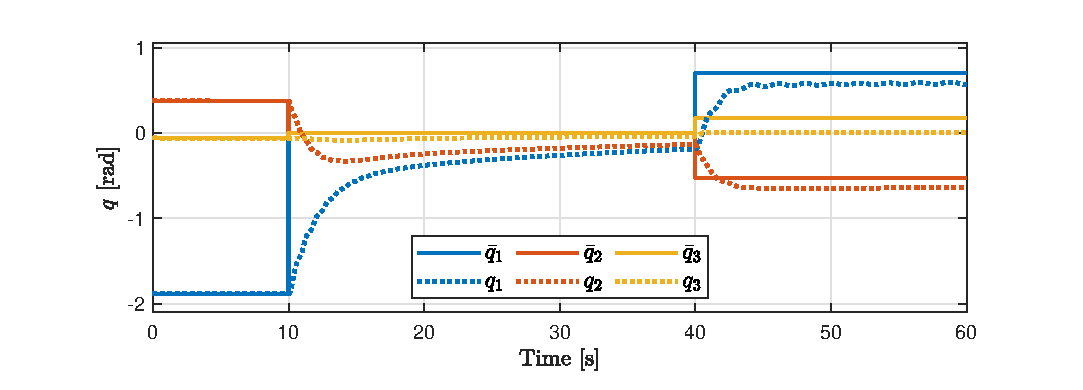
\includegraphics[width=0.49\textwidth, trim={0.75cm 0.87cm 0.75cm 0cm}]{backstepping/figures/time_series_plot_configuration_full_system_PID_v2}}
  \subfigure{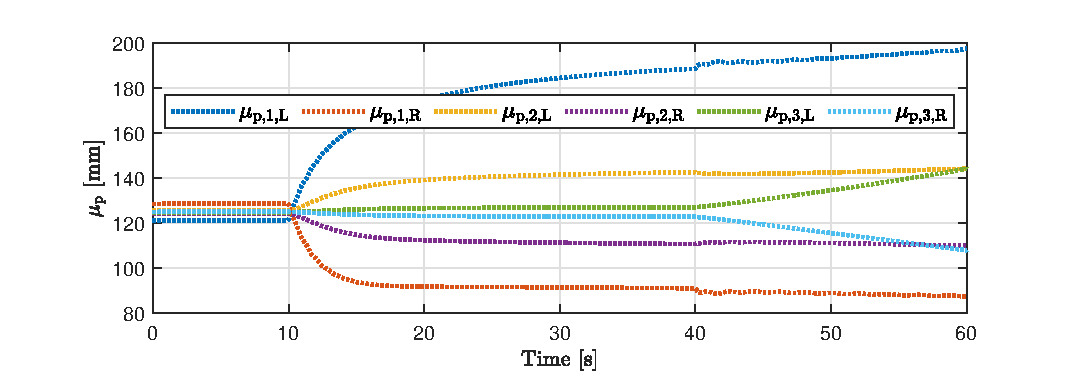
\includegraphics[width=0.49\textwidth, trim={0.75cm 0.87cm 0.75cm 0cm}]{backstepping/figures/time_series_plot_piston_position_full_system_PID_v2.eps}}\\
  % Coupling-aware PID
  \subfigure{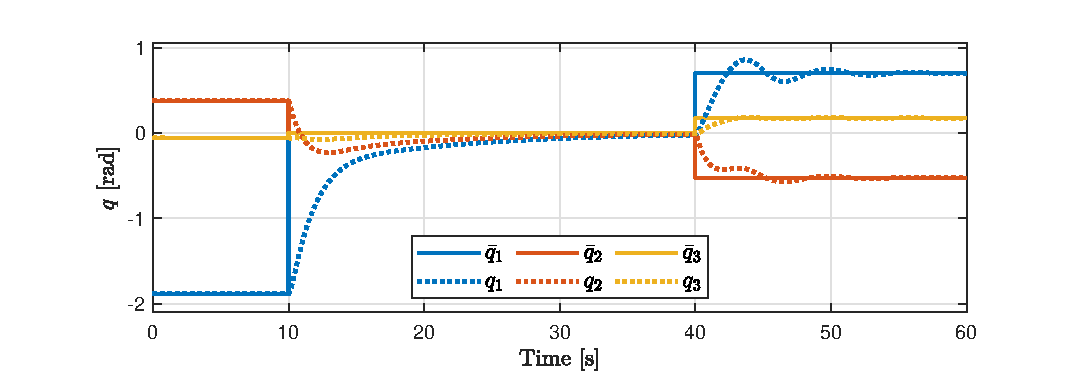
\includegraphics[width=0.49\textwidth, trim={0.75cm 0.87cm 0.75cm 0cm}]{backstepping/figures/time_series_plot_configuration_coupling_aware_PID_v2.eps}}
  \subfigure{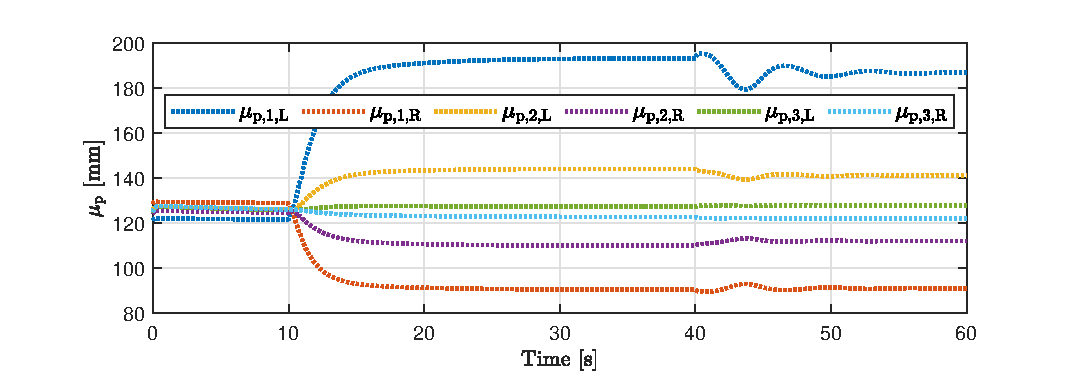
\includegraphics[width=0.49\textwidth, trim={0.75cm 0.87cm 0.75cm 0cm}]{backstepping/figures/time_series_plot_piston_position_coupling_aware_PID_v2.eps}}\\
  % Backstepping
  \setcounter{subfigure}{0}
  \subfigure[Configuration $q$]{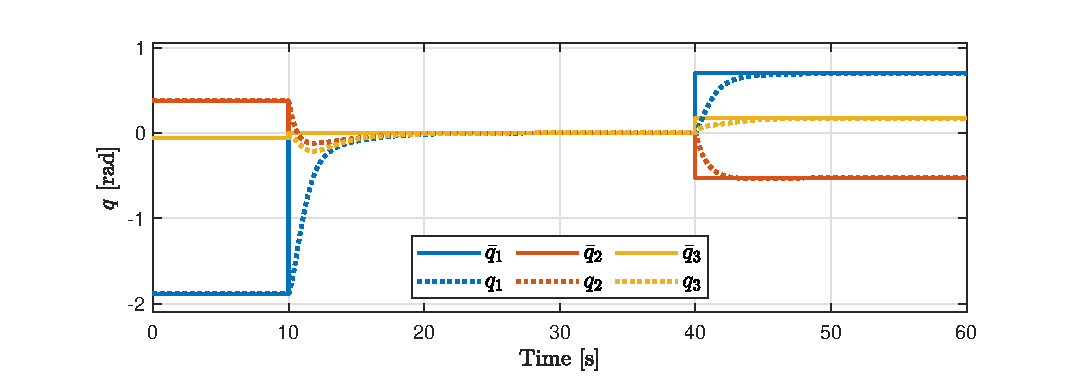
\includegraphics[width=0.49\textwidth, trim={0.75cm 0cm 0.75cm 0cm}]{backstepping/figures/time_series_plot_configuration_backstepping_v2.eps}}
  \subfigure[Piston position $\mu_\mathrm{p}$]{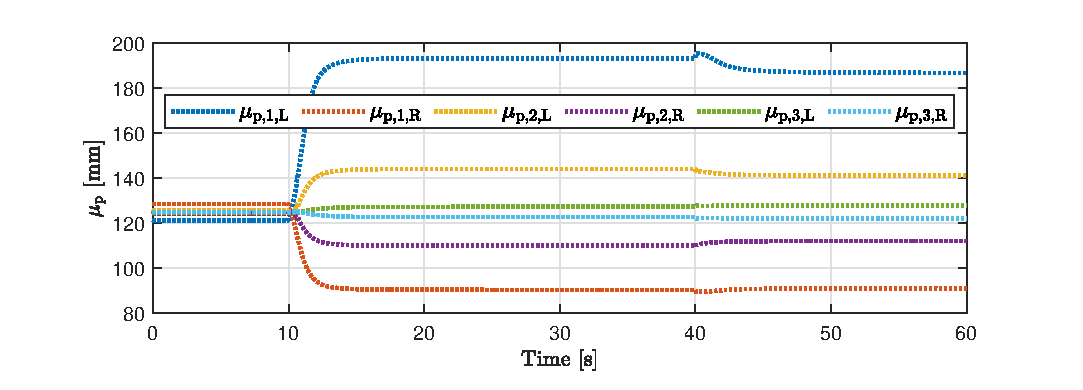
\includegraphics[width=0.49\textwidth, trim={0.75cm 0cm 0.75cm 0cm}]{backstepping/figures/time_series_plot_piston_position_backstepping_v2.eps}}\\
  \caption{Simulation of posture regulation under \gls{PCC} approximation comparing the performance of an end-to-end PID baseline controller (1st row), with a coupling-aware PID controller (2nd row) and the nonlinear backstepping controller (3rd row). The set-point reference configuration is shown with solid lines.}
  \label{fig:backstepping:time_series_plots}
\end{figure}
\begin{figure}[ht]
  \centering
  % End-to-end PID
  \subfigure[End-to-end PID (baseline)]{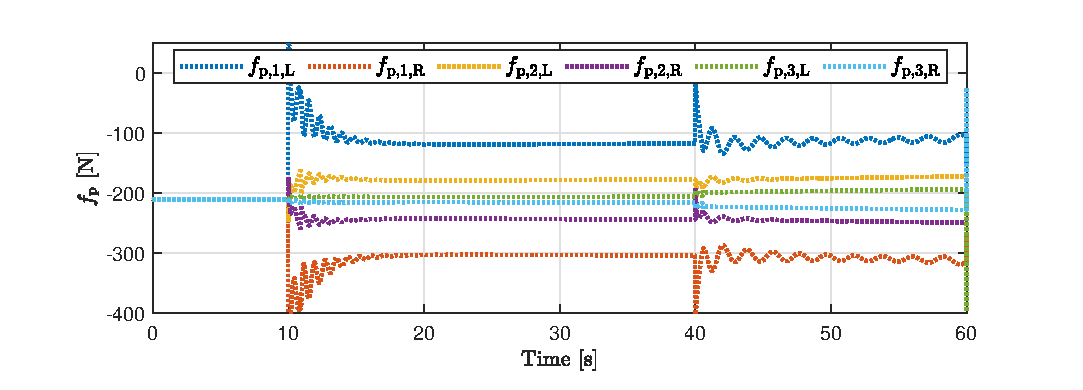
\includegraphics[width=0.49\textwidth, trim={0.75cm 0.0cm 0.75cm 0cm}]{backstepping/figures/time_series_plot_actuation_force_full_system_PID_v2.eps}}
  % Coupling-aware PID
  \subfigure[Coupling-aware PID]{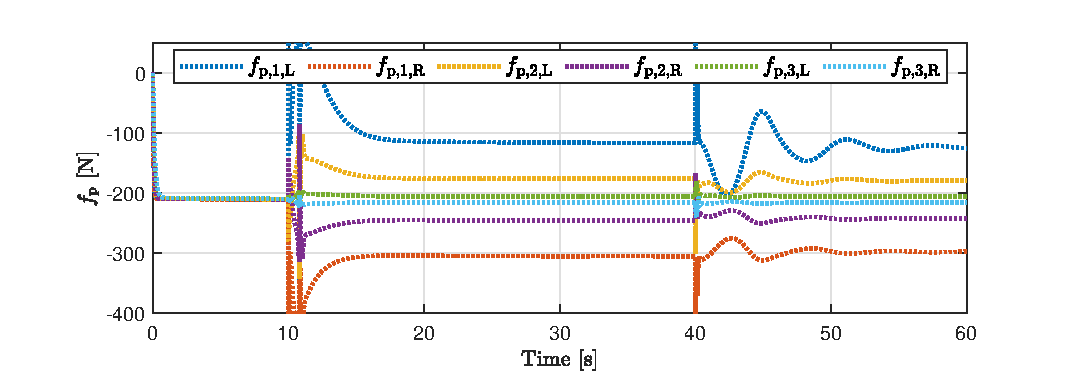
\includegraphics[width=0.49\textwidth, trim={0.75cm 0.0cm 0.75cm 0cm}]{backstepping/figures/time_series_plot_actuation_force_coupling_aware_PID_v2.eps}}\\
  % Backstepping
  \subfigure[Backstepping controller]{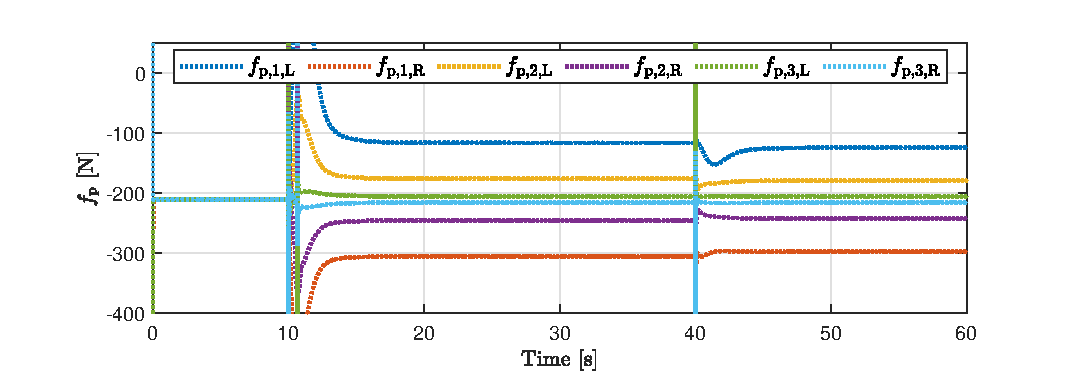
\includegraphics[width=0.49\textwidth, trim={0.75cm 0cm 0.75cm 0cm}]{backstepping/figures/time_series_plot_actuation_force_backstepping_v2.eps}}\\
  \caption{Simulation of posture regulation under \gls{PCC} approximation comparing the control input (i.e., the piston actuation force $f_\mathrm{p}$) of an end-to-end PID baseline controller, a coupling-aware PID controller, and the nonlinear backstepping controller.}
  \label{fig:backstepping:time_series_plots_actuation_force}
\end{figure}

\textbf{Configuration-space control:}
%
Consider the following regulator of desired configuration $\Bar{q} \in \mathbb{R}^{n_\mathrm{q}}$, 
%
\begin{equation}\label{eq:backstepping:high_level_regulation}
    \Bar{\tau}(q, \Bar{q}) = K \Bar{q} + G(q),
\end{equation}
%
where $\Bar{\tau} \in \mathbb{R}^{n_\mathrm{q}}$ is the torque in configuration space. %This will be our high level controller $\Gamm(q)$ as 
%
% This leads to the following equations of motion for the system: %
% \begin{equation}
%      M(q) \Ddot{q} + C(q, \dot{q}) \dot{q} = K (\Bar{q} - q) + D (-\dot{q}),
% \end{equation}
% which is essentially a PD controller with gravity compensation. 
Asymptotic stability of the equilibrium $\Bar{q}$ is proven through the Lyapunov function $H(q, \dot{q}) = \dot{q}^{\top} M(q) \dot{q}/2 + q^\top K q/2$, which yields the time derivative $\dot{H} = -\dot{q}^\top D \dot{q}/2 \leq 0$.

\textbf{Mapping from configuration to actuation space with force balance:}
Our backstepping controller requires access to $\Gamma(q,\dot{q})$ which returns a desired piston $\bar{\mu}_\mathrm{p}$ given the desired torque $\bar{\tau}$ and the current state of the soft system $(q,\dot{q})$. In the planar case with inextensible segments, there exists a redundancy in actuating the pistons controlling the pressure in the left and right chambers of a segment to trigger $\bar{\tau}$ on the segment. Thus, we decide to solve this redundancy by equally attributing the desired torque to both pistons.

We assume that the system is calibrated at a straight configuration $q_{\mathrm{t}0} = 0$ with pistons preloaded at position $\mu_{p,t0} \in \mathbb{R}^{n_{\mu_\mathrm{p}}}$ leading to a fluidic volume of
 \begin{equation}
     V_{\mathrm{t}0,j} = V_{\mathrm{C},j}(q_{\mathrm{t}0,i}) + \mu_{\mathrm{p},\mathrm{t}0,j} \, A_{\mathrm{p},j}
 \end{equation}
 % and causing a fluidic pressure of $p_{\mathrm{t}0,j} = p_\mathrm{atm} \frac{V_{\mathrm{C},j}(q_i=0) + l_{\mathrm{p},j} A_{\mathrm{p},j}}{V_{\mathrm{C},j}(q_i=0) + \mu_{\mathrm{p},\mathrm{t}0,j} A_{\mathrm{p},j}}$ 
in the system. After preloading, the fluids in the left and right chambers each apply a preloaded torque of magnitude $G_{\mathrm{P},\mathrm{t}0}^{q} \in \mathbb{R}^{n_\mathrm{q}}$ on the soft system.
% \begin{equation}
%     G_{\mathrm{P},\mathrm{t}0,i}^{q} =
%     -p_\mathrm{atm} \partial_{q_i} V_{\mathrm{C},j} A_{\mathrm{p},j} \frac{l_{\mathrm{p},j} - \mu_{\mathrm{p},\mathrm{t}0,j}}{V_{\mathrm{t}0,j}}.
% \end{equation}
It is implicitly assumed that the piston length $l_\mathrm{p}$, piston area $A_\mathrm{p}$, the preloaded piston position $\mu_{\mathrm{p},\mathrm{t}0}$ and the preloaded volume $V_{\mathrm{t}0}$ are equal for the left and right chambers of segment $i$.
We can write the conservative forces acting on the left chamber $G_{\mathrm{P},\mathrm{L}}^q(q, \mu_\mathrm{p}) \in \mathbb{R}^{n_\mathrm{q}}$ and right chamber $G_{\mathrm{P},\mathrm{R}}^q(q, \mu_\mathrm{p}) \in \mathbb{R}^{n_\mathrm{q}}$ as differences from the neutral conservative force $G_{\mathrm{P},\mathrm{t}0}^{q}$
\begin{equation}
\begin{split}
    G_{\mathrm{P},\mathrm{L}}^q = G_{\mathrm{P},\mathrm{t}0}^{q} + \Delta G_{\mathrm{P},\mathrm{L}}^q,
    \quad
    G_{\mathrm{P},\mathrm{R}}^q = - G_{\mathrm{P},\mathrm{t}0}^{q} + \Delta G_{\mathrm{P},\mathrm{R}}^q.
\end{split}
\end{equation}
% \begin{equation}
% \begin{split}
%     G_{\mathrm{P},\mathrm{L}}^q(q, \mu_\mathrm{p}) &= G_{\mathrm{P},\mathrm{t}0}^{q} + \Delta G_{\mathrm{P},\mathrm{L}}^q(q, \mu_\mathrm{p}),\\
%     G_{\mathrm{P},\mathrm{R}}^q(q, \mu_\mathrm{p}) &= - G_{\mathrm{P},\mathrm{t}0}^{q} + \Delta G_{\mathrm{P},\mathrm{R}}^q(q, \mu_\mathrm{p}).
% \end{split}
% \end{equation}
The force applied by the fluid in the left and right chambers on the system is
\begin{equation}
    G_{\mathrm{P}}^q(q, \mu_p) =  G_{\mathrm{P},\mathrm{L}}^q + G_{\mathrm{P},\mathrm{R}}^q = \Delta G_{\mathrm{P},\mathrm{L}}^q + \Delta G_{\mathrm{P},\mathrm{R}}^q .
\end{equation}
We re-arrange to find an expression for the desired conservative force offsets, which equally distribute a commanded torque $\Bar{\tau}$ to the fluid in both chambers. Setting
$\Delta \Bar{G}_{\mathrm{P},\mathrm{L}}^{\Bar{q}} =  \Delta \Bar{G}_{\mathrm{P},\mathrm{R}}^{\Bar{q}} = 0.5 \, \Bar{\tau}(q, \Bar{q})$
% \begin{equation}
%      \Delta \Bar{G}_{\mathrm{P},\mathrm{L}}^{\Bar{q}} =  \Delta \Bar{G}_{\mathrm{P},\mathrm{R}}^{\Bar{q}} = 
%      % -\frac{\Bar{\tau}}{2},
%      0.5 \, \Bar{\tau}(q, \Bar{q}),
% \end{equation}
results for the chosen setpoint controller $\Bar{\tau}$ and a diagonal elastic matrix $K$ with elements $k_i$ in:
\begin{equation}\label{eq:backstepping:dist_G_p_q_planar_pcc}
    \Bar{G}_{\mathrm{P},j}^{\Bar{q}}(q, \Bar{q}_i) 
    % = \pm G_{\mathrm{P},\mathrm{t}0,i}^{q} - 0.5 \Bar{\tau}_i 
    = \pm G_{\mathrm{P},\mathrm{t}0,i}^{q} - 0.5 \left ( k_i \Bar{q}_i + G_i(q) \right ).
\end{equation}
Eq.~\eqref{eq:backstepping:GPmu} is inversed to compute the desired piston position $\Bar{\mu}_{\mathrm{p}} = \Gamma(q, \Bar{q})$:
\begin{equation}\label{eq:backstepping:gamma}
    \Gamma_j(q, \Bar{q}) = \frac{1}{A_{\mathrm{p},j}} \left ( \frac{\alpha_{\mathrm{air},j} \, \partial_{q_i} V_{\mathrm{C},j}}{p_\mathrm{atm} \, \partial_{q_i} V_{\mathrm{C},j} - \Bar{G}_{\mathrm{P},j}^{\Bar{q}}(q, \Bar{q})} - V_{\mathrm{C},j}(q) \right ).
\end{equation}
\textbf{Backstepping:}
The system is now in the form of Eq.~\eqref{eq:backstepping:reduced_sys}, so Theorem~1 can be invoked and a specialized version of Eq.~\eqref{eq:backstepping:pi_psi} can be derived for the \gls{PCC}-case and our chosen set-point controller of Eq.~\eqref{eq:backstepping:high_level_regulation}. The partial derivative of the Lyapunov function of the soft system controller evaluates to $ \partial_{\dot{q}} H(q, \dot{q}) = \dot{q}^\top M(q)$, which allows to re-formulate \eqref{eq:backstepping:pi_psi} into:
\begin{equation}\small
\begin{split}
    \bar{\dot{\mu}}_\mathrm{p} = \Pi(q,\dot{q},\mu_\mathrm{p}) &= \dot{\Gamma}(q,\dot{q}) - K_1 (\mu_p - \Gamma(q)) + S^\top(q,\mu_\mathrm{p},\Gamma(q)) \, \dot{q},\\
    \bar{f}_\mathrm{p} = \Psi(q,\dot{q},\mu_\mathrm{p}, \dot{\mu}_\mathrm{p}) &= G_{\mathrm{P}}^{\mu_\mathrm{p}} + D_\mathrm{p} \, \Pi(q,\dot{q},\mu_\mathrm{p}) + M_\mathrm{p} \, \dot{\Pi} - K_2 \, (\dot{\mu}_\mathrm{p} - \Pi(q,\dot{q},\mu_\mathrm{p})) - (\mu_\mathrm{p} - \Gamma(q)).
\end{split}
\end{equation}

% \textbf{Backstepping to piston velocity:} 
% To complete the backstepping to the piston velocity $\Pi(q, \dot{q})$, we require access to the time derivative of the \gls{PCC} controller in actuation space $\dot{\Gamma}(q, \Bar{q}, \dot{q}) = \partial_q \Gamma (q, \Bar{q}) \dot{q}$:
% \begin{equation}
%     \dot{\Gamma}_j = \frac{1}{A_{\mathrm{p},j}} \left ( \frac{\alpha_{\mathrm{air},j} \partial_{q_i} V_{\mathrm{C},j} \partial_{q} \Bar{G}_{\mathrm{P},j}^{\Bar{q}}}{\left ( p_\mathrm{atm} \partial_{q_i} V_{\mathrm{C},j} - \Bar{G}_{\mathrm{P},j}^{\Bar{q}} (q, \Bar{q}) \right )^2} - \partial_{q} V_{\mathrm{C},j} \right ) \dot{q}.
% \end{equation}
% For the proposed setpoint controller, we can subsequently also determine the partial derivative of the commanded force $\partial_q \Bar{G}_{\mathrm{P},j}^{\Bar{q}}(q, \Bar{q}) = - 0.5 \, \partial_q G_i(q)$.
% The partial derivative of the Lyapunov function of the soft system controller evaluates to $ \partial_{\dot{q}} H(q, \dot{q}) = \dot{q}^\top M(q)$, which allows us to re-formulate \eqref{eq:backstepping:pi_psi}:
% \begin{equation}\label{eq:backstepping:pi_pcc_set_point}
%     \Pi(q, \Bar{q}, \dot{q}, \mu_\mathrm{p}) = \dot{\Gamma} - K_1 (\mu_p - \Gamma) + S^\top \dot{q}.
% \end{equation}
% \textbf{Backstepping to piston force:}
% We require access to the time derivative of the controller $\Pi(q, \dot{q})$:
% \begin{equation}
%     \dot{\Pi}(q, \Bar{q}, \dot{q}, \mu_\mathrm{p}, \dot{\mu}_\mathrm{p}) = \partial_q \Pi \dot{q} + \partial_{\dot{q}} \Pi \Ddot{q} + \partial_{\mu_\mathrm{p}} \Pi \dot{\mu}_\mathrm{p},
% \end{equation}
% and substitute $\Ddot{q} = f(q, \dot{q}) + g(q, \mu_\mathrm{p})$ as accelerations are hard to measure in reality
% \begin{equation}
% \begin{split}
%     \dot{\Pi} = & -K_1 \left ( \dot{\mu}_\mathrm{p} - \dot{\Gamma}(q, \Bar{q}, \dot{q}) \right ) + \left ( \partial_q \dot{\Gamma} + \dot{S}^\top \right ) \dot{q}\\
%     & + \left ( \partial_{\dot{q}} \dot{\Gamma} + S^\top \right ) \left ( f(q,\dot{q}) + g(q,\mu_\mathrm{p}) \right ) .
% \end{split}
% \end{equation}
% We define the final controller of the required piston force $\Bar{f}_\mathrm{p}$
% \begin{equation}
% \begin{split}
%     & \Bar{f}_\mathrm{p} = \Psi(q, \Bar{q}, \dot{q}, \mu_\mathrm{p}, \dot{\mu}_\mathrm{p})\\
%     & \Psi = G_{\mathrm{P}}^{\mu_\mathrm{p}} + D_\mathrm{p} \, \Pi + M_\mathrm{p} \, \dot{\Pi} - K_2 \, (\dot{\mu}_\mathrm{p} - \Pi) - (\mu_\mathrm{p} - \Gamma).
% \end{split}
% \end{equation}
\section{Simulations}
%
% \begin{figure*}[ht]
%   \centering
%   \subfigure[Configuration $q$]{\includegraphics[width=0.33\textwidth]{figures/time_series_plot_m_p-0.5_untuned_configuration_v2.eps}\label{fig:backstepping:time_series_plot_m_p_0.5_configuration}}
%   \subfigure[Piston position $\mu_\mathrm{p}$]{\includegraphics[width=0.33\textwidth]{figures/time_series_plot_m_p-0.5_untuned_piston_position_v2.eps}\label{fig:backstepping:time_series_plot_m_p_0.5_piston_position}}
%   \subfigure[Actuation force $f_\mathrm{p}$]{\includegraphics[width=0.33\textwidth]{figures/time_series_plot_m_p-0.5_untuned_actuation_force_v2.eps}\label{fig:backstepping:time_series_plot_m_p_0.5_actuation_force}}\\
%   \caption{Simulation of posture regulation under \gls{PCC} approximation for an actuation system with increased inertia ($m_\mathrm{p} = \SI{0.5}{kg}$) comparing the performance of the nonlinear backstepping controller (dashed lines) with a PID baseline controller (dotted lines). The set-point reference configuration is shown with solid lines. All gains remain unchanged and are tuned for the original system with $m_\mathrm{p} = \SI{0.19}{kg}$.}
% \end{figure*}
\begin{figure}[ht]
  \centering
  % End-to-end PID
  \subfigure{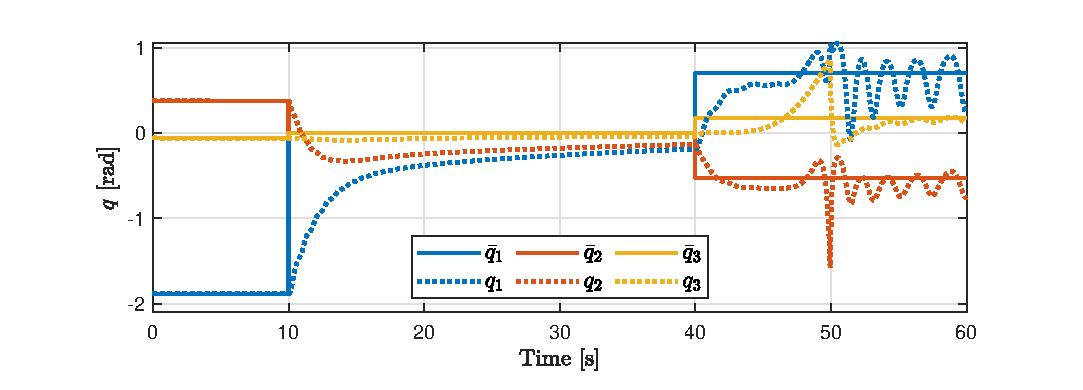
\includegraphics[width=0.49\textwidth, trim={0.75cm 0.85cm 0.75cm 0cm}]{backstepping/figures/time_series_plot_m_p-0.5_untuned_configuration_full_system_PID_v2.eps}}
  \subfigure{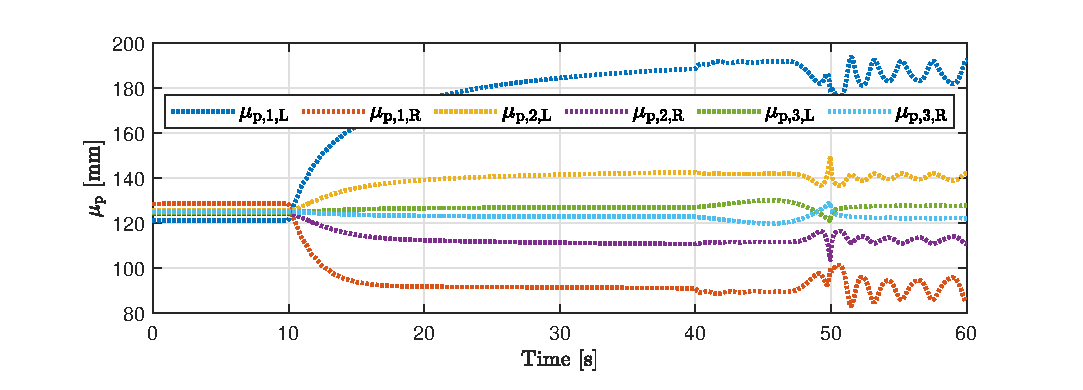
\includegraphics[width=0.49\textwidth, trim={0.75cm 0.85cm 0.75cm 0cm}]{backstepping/figures/time_series_plot_m_p-0.5_untuned_piston_position_full_system_PID_v2.eps}}
  % Coupling-aware PID
  \subfigure{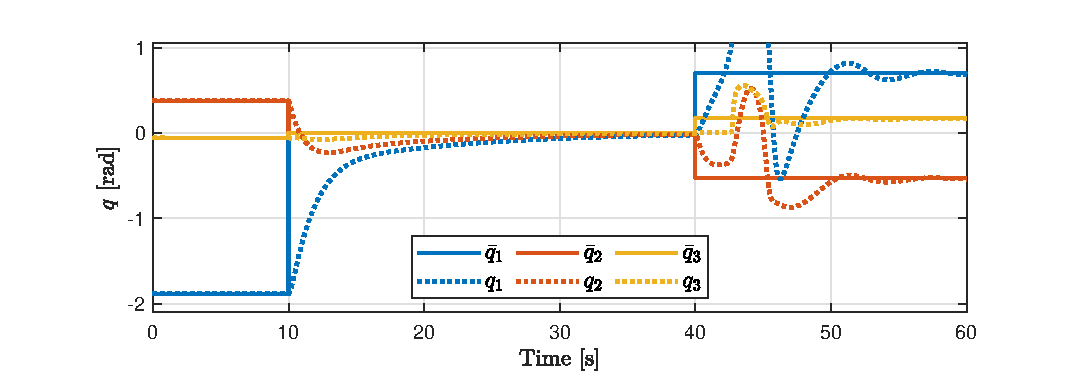
\includegraphics[width=0.49\textwidth, trim={0.75cm 0.85cm 0.75cm 0cm}]{backstepping/figures/time_series_plot_m_p-0.5_untuned_configuration_coupling_aware_PID_v2.eps}}
  \subfigure{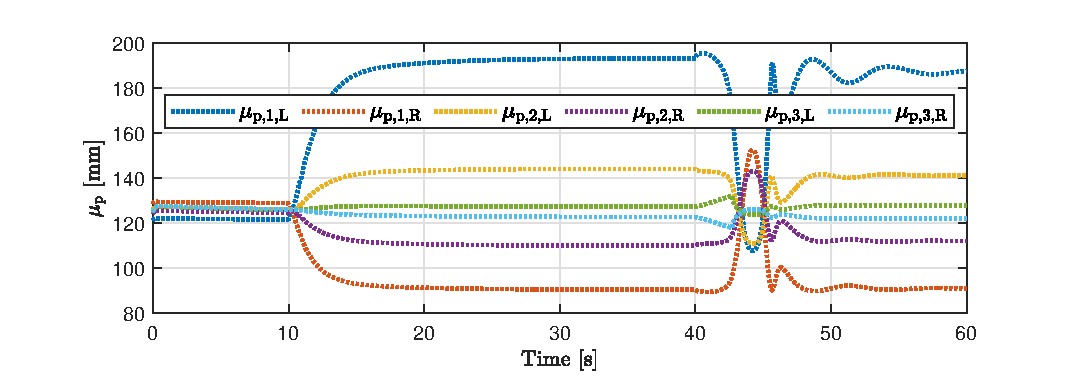
\includegraphics[width=0.49\textwidth, trim={0.75cm 0.85cm 0.75cm 0cm}]{backstepping/figures/time_series_plot_m_p-0.5_untuned_piston_position_coupling_aware_PID_v2.eps}}
  % Backstepping
  \setcounter{subfigure}{0}
  \subfigure[Configuration $q$]{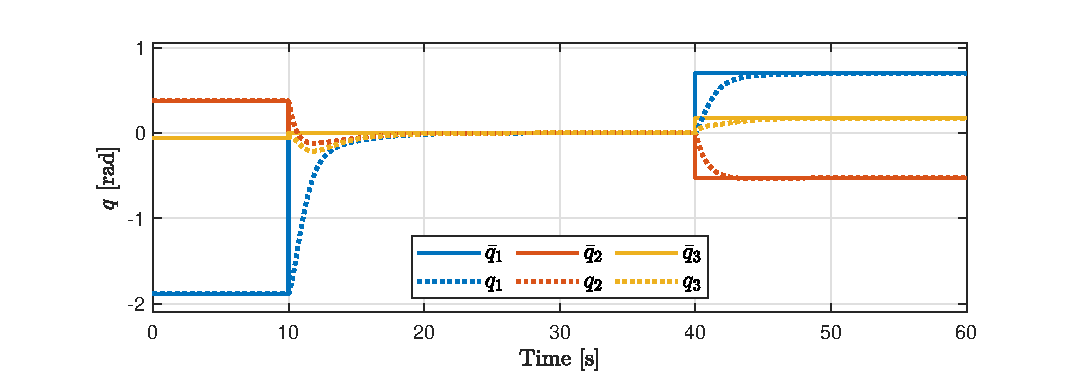
\includegraphics[width=0.49\textwidth, trim={0.75cm 0cm 0.75cm 0cm}]{backstepping/figures/time_series_plot_m_p-0.5_untuned_configuration_backstepping_v2.eps}}
  \subfigure[Piston position $\mu_\mathrm{p}$]{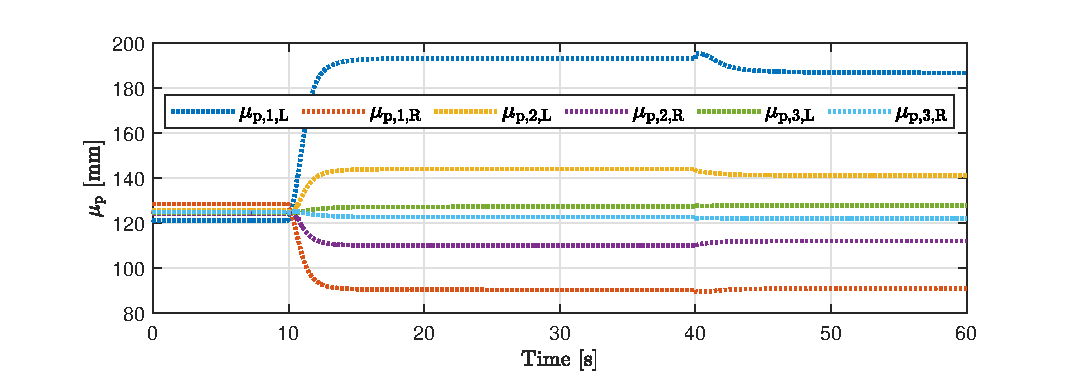
\includegraphics[width=0.49\textwidth, trim={0.75cm 0cm 0.75cm 0cm}]{backstepping/figures/time_series_plot_m_p-0.5_untuned_piston_position_backstepping_v2.eps}}
  \caption{Simulation of posture regulation under \gls{PCC} approximation for an actuation system with increased inertia ($m_\mathrm{p} = \SI{0.5}{kg}$) comparing the performance of an end-to-end PID baseline controller (1st row), with a coupling-aware PID controller (2nd row) and the nonlinear backstepping controller (3rd row). The set-point reference configuration is shown with solid lines.}
  \label{fig:backstepping:time_series_plots_m_p-0.5_untuned}
\end{figure}
\begin{figure}[ht]
  \centering
  % End-to-end PID
  \subfigure[End-to-end PID (baseline)]{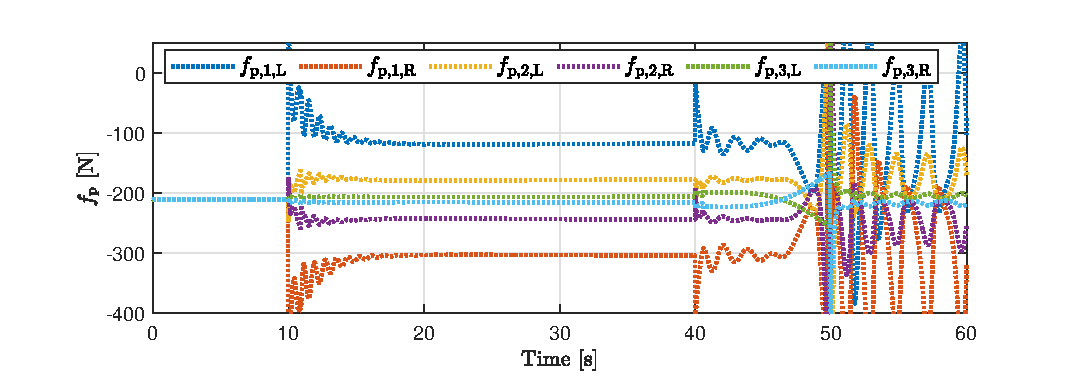
\includegraphics[width=0.49\textwidth, trim={0.75cm 0.0cm 0.75cm 0cm}]{backstepping/figures/time_series_plot_m_p-0.5_untuned_actuation_force_full_system_PID_v2.eps}}
  % Coupling-aware PID
  \subfigure[Coupling-aware PID]{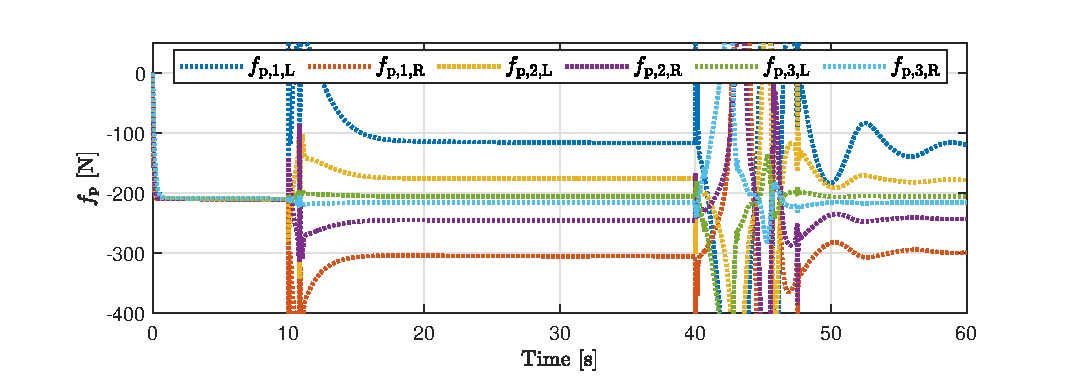
\includegraphics[width=0.49\textwidth, trim={0.75cm 0.0cm 0.75cm 0cm}]{backstepping/figures/time_series_plot_m_p-0.5_untuned_actuation_force_coupling_aware_PID_v2.eps}}\\
  % Backstepping
  \subfigure[Backstepping controller] {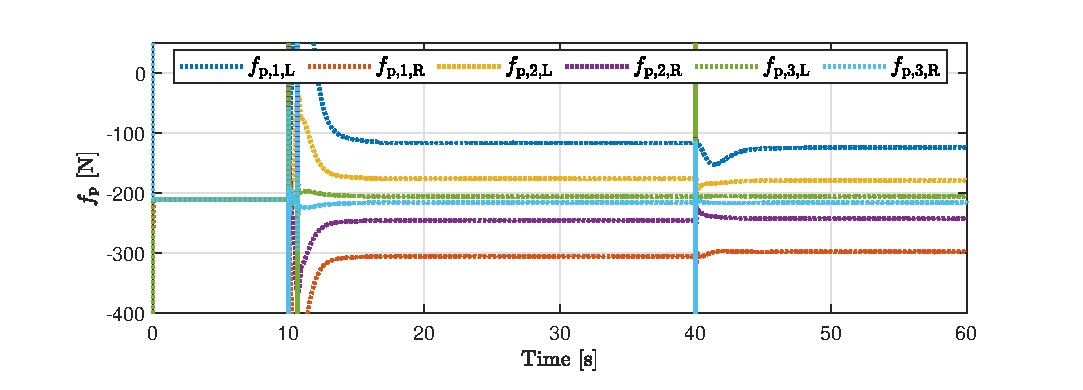
\includegraphics[width=0.49\textwidth, trim={0.75cm 0cm 0.75cm 0cm}]{backstepping/figures/time_series_plot_m_p-0.5_untuned_actuation_force_backstepping_v2.eps}}\\
  \caption{Simulation of posture regulation under \gls{PCC} approximation for an actuation system with increased inertia ($m_\mathrm{p} = \SI{0.5}{kg}$) comparing the control input (i.e., the piston actuation force $f_\mathrm{p}$]) of an end-to-end PID baseline controller, of a coupling-aware PID controller and the nonlinear backstepping controller.}
  \label{fig:backstepping:time_series_plots_m_p-0.5_untuned_actuation_force}
\end{figure}
%
\begin{figure}[ht]
  \centering
  \subfigure[End-to-end PID]{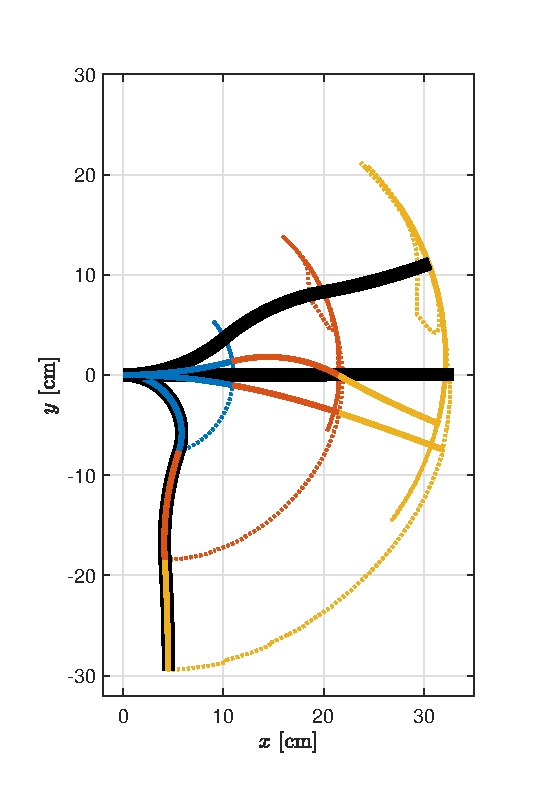
\includegraphics[width=0.32\columnwidth, trim={0.5cm 0 0.5cm 0}]{backstepping/figures/cartesian_evolution_plot_m_p-0.5_untuned_full_system_pid_v1.eps}\label{fig:backstepping:cartesian_evolution_plot_m_p-0.5_untuned_full_system_pid}}
  \subfigure[Coupling-aware PID]{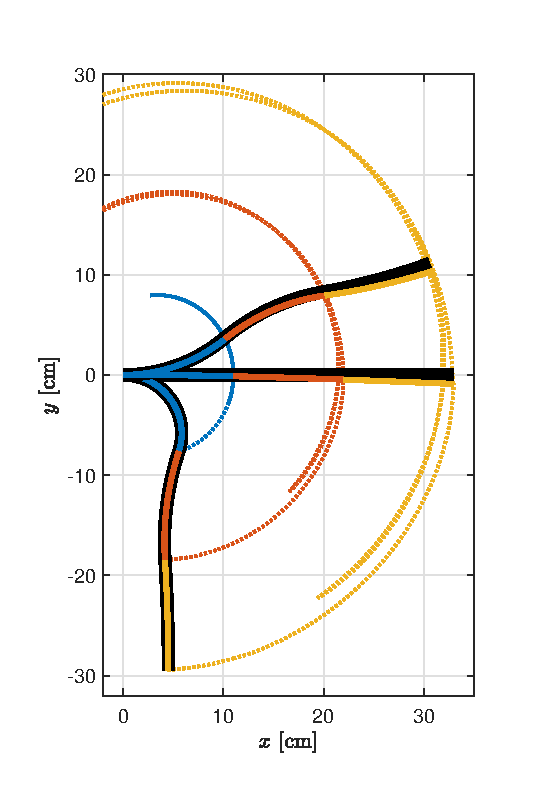
\includegraphics[width=0.32\columnwidth, trim={0.5cm 0 0.5cm 0}]{backstepping/figures/cartesian_evolution_plot_m_p-0.5_untuned_coupling_aware_pid_v1.eps}\label{fig:backstepping:cartesian_evolution_plot_m_p-0.5_untuned_coupling_aware_pid}}
  \subfigure[Backstepping]{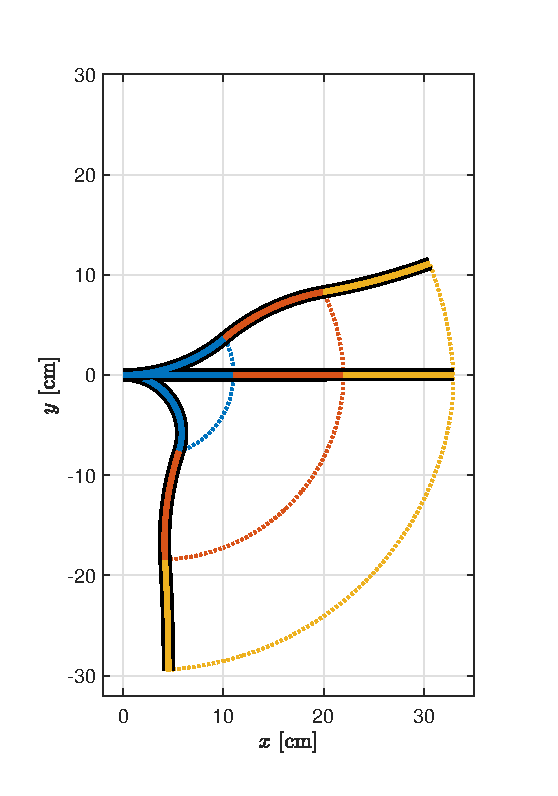
\includegraphics[width=0.32\columnwidth, trim={0.5cm 0 0.5cm 0}]{backstepping/figures/cartesian_evolution_plot_m_p-0.5_untuned_backstepping_v2.eps}\label{fig:backstepping:cartesian_evolution_plot_m_p-0.5_untuned_backstepping}}
  \caption{Cartesian evolution of the soft robot for an actuation system with increased inertia ($m_\mathrm{p} = \SI{0.5}{kg}$). All gains remain unchanged and are tuned for the original system with $m_\mathrm{p} = \SI{0.19}{kg}$. The dotted lines mark the evolution of the tip of the segments. The soft robot consists of three segments (blue, orange, and yellow). The reference configuration at the three set points is marked with a thick black line.}\label{fig:backstepping:cartesian_evolution_plot_m_p-0.5_untuned}
\end{figure}
%
\subsection{System}
%
We consider a planar soft robot arm consisting of three independently actuated CC segments, modeled upon the second half of the robot in \citep{della2020model}. % in Simulink. It is inspired by recent designs and models of similar pneumatically actuated continuum arms in literature~\citep{della2020model, marchese2014design}. 
%We model the 
Segments have equal length $l_{0} = \SI{11}{cm}$, uniform mass density $\rho = \SI{0.99}{kg \per m}$ concentrated on the central axis. % - resulting in \SI{109}{g} per segment. %We use the \gls{PCC} assumption~\citep{jones2006kinematics} to compute the Jacobian for any point along the center-line of the segment. The \gls{EoM} are derived using the Euler-Lagrange equation. We add an elastic term $K q$ with $K$ defined as a diagonal matrix with the elastic constant \SI{0.01}{N \per rad}. Natural damping is considered with $D \dot{q}$ and the diagonal damping constant \SI{0.01}{Ns \per rad}.
%
The stiffness $K$ and damping $D$ matrices are diagonal with constants \SI{0.01}{N \per rad} and \SI{0.01}{Ns \per rad}. The segment has a diameter of \SI{44.5}{mm}. Based on CAD analyses of a real system, we take $d_{\mathrm{C},\mathrm{a}} = \SI{7.14}{mm}$, $d_{\mathrm{C},\mathrm{b}} = \SI{20.19}{mm}$, and $b_\mathrm{C} = \SI{8.07}{mm}$.
%We set the parameters $d_{\mathrm{C},\mathrm{a}}$ and $d_{\mathrm{C},\mathrm{b}}$ as the inner and outer air chamber walls are placed at a radial distance of \SI{7.14}{mm} and \SI{20.19}{mm}. We analysed the chamber volume in CAD to be \SI{46.2}{cm^3}, which results in a modelled planar chamber depth of $b_\mathrm{C} = \SI{8.07}{mm}$.
%
%The base of the first segment is aligned with the x-axis and gravity is acting along the negative y-axis. 
A positive curvature and positive configuration $q_i$ correspond to bending counter-clockwise. 
% The base of the robot is oriented perpendicularly to gravity, so that it tends to induce clock-wise bending.
The straight configuration of the robot along the x-axis is perpendicular to gravity acting in the negative y-direction, as shown in Figure~\ref{fig:backstepping:pcc_case_overview}, so that gravity tends to induce clockwise bending.
%
%We were inspired by the fluidic drive cylinder designed by \citet{marchese2014design} in our choice of parameters for the pistons. Accordingly, 
Moving to the pistons, $A_\mathrm{p} = \SI{7.9}{cm^2}$, $m_\mathrm{p} = \SI{0.19}{kg}$, $l_\mathrm{p} = \SI{0.5}{m}$ are chosen.
% We model the cross-sectional area of the piston $A_\mathrm{p}$ as \SI{7.9}{cm^2}, the mass of the piston $m_\mathrm{p}$ with \SI{0.19}{kg} resulting in a diagonal mass matrix $M_\mathrm{p}$, the length of the piston $l_\mathrm{p}$ as \SI{0.5}{m} and 
We consider a damping matrix $D_\mathrm{p}$ with damping constants $d_\mathrm{p} = \SI{10}{\kilo \newton \second \per \meter}$ along the diagonal. The pistons are filled with air at $\mu_{\mathrm{p}, 0} = l_\mathrm{p}$ and $p_\mathrm{atm} = \SI{1}{bar}$ and subsequently pre-loaded to $\mu_{\mathrm{p}, \mathrm{t}0} = 0.25 \, l_\mathrm{p}$. % before the experiment is started.
We set the backstepping gains to $K_1 = \SI{6000}{\per \second}$ and $K_2 = \SI{4.5}{\kilo \newton \per \meter}$.

\subsection{End-to-End PID}
We first introduce an end-to-end PID controller, which will serve as a baseline
%
\begin{equation}
    \Delta f_\mathrm{p} = K_\mathrm{p} (\bar{q}-q) + K_\mathrm{i} \int_0^t (\bar{q}-q) \, \mathrm{d}t' - K_\mathrm{d} \, \dot{q}
\end{equation}
%
where $K_\mathrm{p},K_\mathrm{i},K_\mathrm{d} \geq 0$ are scalar gains. $\Delta f_\mathrm{p} \in \mathbb{R}^{n_q}$ is the scalar offset from the actuation force $f_{\mathrm{p},\mathrm{t}0}$ corresponding to the pre-loaded pressure $p_{\mathrm{t}0}$.
%
Analog to \eqref{eq:backstepping:dist_G_p_q_planar_pcc}, $\Delta f_\mathrm{p}$ can be equally distributed on both chambers within a segment.
% \begin{equation}
% \begin{split}
%     f_{\mathrm{p},\mathrm{L},i} = f_{\mathrm{p},\mathrm{t}0} + 0.5 \, \Delta f_{\mathrm{p},i}, \quad f_{\mathrm{p},\mathrm{R},i} = f_{\mathrm{p},\mathrm{t}0} - 0.5 \, \Delta f_{\mathrm{p},i}.
% \end{split}
% \end{equation}
The PID gains have been selected so to achieve a similar transient behavior as for the backstepping controller % required lengthy heuristic tuning and the selection was guided by the Ziegler-Nichols method,
and are equal to $K_\mathrm{p} = \SI{200}{\newton \per \radian}$, $K_\mathrm{i} = \SI{7}{\newton \per \radian \per \second}$, and $K_\mathrm{d} = \SI{200}{\newton \second \per \radian}$. 
% Segment 1, 2 and 3 are weighted with gain multipliers of $1.5$, $1$, and $0.5$.

%
\subsection{Coupling-Aware PID}
%
% We attempted implementing a standard low-level PID with static compensation as in \citep{della2020model} for fair comparison, but we could not find a set of gains that was stable when using \eqref{eq:backstepping:high_level_regulation}.
Next, we implement a control strategy that takes advantage of the understanding of the potential coupling and uses a PID for low-level control of the pistons
%
\begin{equation}
    f_{\mathrm{p}} = K_\mathrm{p} \left (\Gamma(q, \bar{q})-\mu_\mathrm{p} \right ) +  K_\mathrm{i} \int_{0}^t \left ( \Gamma(q, \bar{q})-\mu_\mathrm{p} \right ) \mathrm{d}t' - K_\mathrm{d} \, \dot{\mu}_\mathrm{p}.
\end{equation}
%
Here, $K_\mathrm{p},K_\mathrm{i},K_\mathrm{d} \geq 0$ are scalar gains, and $\Gamma(q, \bar{q})$ is the correction on \eqref{eq:backstepping:high_level_regulation} which takes the coupling defined in \eqref{eq:backstepping:gamma} in account. 
%
The PID gains are tuned similarly to the coupling-aware PID
and are equal to $K_\mathrm{p} = \SI{150 000}{\newton \per \meter}$, $K_\mathrm{i} = \SI{15 000}{\newton \per \meter \per \second}$, and $K_\mathrm{d} = \SI{100}{\newton \second \per \meter}$. 
% Segment 1, 2 and 3 are weighted with gain multipliers of $1.5$, $1$, and $0.5$.  %~\citep{ziegler1942optimum}.

\subsection{Results}

We simulate the response of the closed-loop generated by all three controllers to a sequence of step references. The segments are initialized at the equilibrium configuration. % of the system $\begin{bmatrix} \SI{-1.8850}{\radian} & \SI{0.3752}{\radian} & \SI{-0.0593}{\radian} \end{bmatrix}^\top$, where they are for \SI{10}{s}. 
At \SI{10}{s}, the reference is moved to the straight configuration $\bar{q} =  0$. After another \SI{30}{s}, we change it again to $\bar{q} = \begin{bmatrix} \SI{0.6981}{\radian} & \SI{-0.5236}{\radian} & \SI{0.1745}{\radian} \end{bmatrix}^\top$.
% We choose an \emph{ode45} with variable step size and a max step size of $0.001$ for our Simulink simulation. %To avoid numerical instabilities of the PCC formulation close to a straight configuration, we use $\tilde{q}$  with $\lvert \tilde{q}_i \rvert = \max (q_i, \SI{3}{\degree})$ as the input into the \gls{EoM} and the controller formulations.

Figures~\ref{fig:backstepping:time_series_plots}-\ref{fig:backstepping:time_series_plots_actuation_force} show that the backstepping controller is approaching the set-point reference with no oscillations or overshooting. These are instead visible for coupling-are PID controller after the second change in reference configuration. 
The end-to-end PID controller does not converge to the desired configuration within \SI{60}{s} as it does not take into account gravity.

Next, we increase the inertia of the actuation system by setting the piston mass $m_\mathrm{p}$ to \SI{0.5}{kg}. We leave both the backstepping and the PID gains unchanged. Figures~\ref{fig:backstepping:time_series_plots_m_p-0.5_untuned}-\ref{fig:backstepping:cartesian_evolution_plot_m_p-0.5_untuned} demonstrate that the backstepping-based approach is able to adapt to the new system, while the end-to-end PID shows large oscillations at \SI{50}{s} and the coupling-aware PID displays significant overshoot in curvatures and piston positions. 
Note that the latter are especially dangerous in real experiments since they may signify that pistons reach their limits.

% \begin{table*}
% \centering
% \caption{System parameters used in simulations}
% \begin{tabular}{c c c c c c c c c c}\toprule
% $l$ & $\rho$ & $k$ & $d$ & $b_\mathrm{C}$ & $d_{\mathrm{C},a}$ & $d_{\mathrm{C},b}$ & $A_\mathrm{p}$ & $l_\mathrm{p}$ & $m_\mathrm{p}$\\
% \midrule
% \SI{110}{mm} & \SI{0.99}{g \per mm} & \SI{0.01}{N \per \radian} & \SI{0.01}{Ns \per \radian} & \SI{8.07}{mm} & \SI{7.14}{mm} & \SI{20.19}{mm} & \SI{7.9}{cm^2}~\citep{marchese2014design} & \SI{0.5}{m} & \SI{0.19}{kg}~\citep{marchese2014design}\\
% \bottomrule
% \end{tabular}
% \label{tab:system_parameters}
% \end{table*}
\section{Conclusion}\label{sec:backstepping:conclusion}
%
This chapter proposed a model for soft robots actuated using pneumatic fluidic drive cylinders and introduced a model-based controller to take the actuators' dynamics into account. The stability of this backstepping-based control strategy was proven using a Lyapunov argument.  As an example of application, model and control strategy have been specialized for the planar \gls{PCC}-case. We also proposed a coupling-aware extension of the standard hierarchical PID strategy as a middle-ground solution.

% Future work will focus on applying this strategy to more sophisticated models and controllers and on experimental validation in a lab environment. 
% Specifically, the model (in particular the the fluidic volume model) and controller should be augmented to allow for control in 3D instead of only in planar settings.
% Also, it would be interesting to investigate if a similar backstepping-based control approach could be applied to the other type of pneumatic actuation - pressure regulation via valve systems.
Future work will focus on extending this strategy to more sophisticated models and controllers while validating it experimentally in a lab environment. In particular, the model—especially the fluidic volume model—and the controller should be enhanced and augmented to enable 3D control rather than being limited to planar settings. Additionally, it would be interesting to explore whether a similar backstepping-based control approach could be applied to alternative pneumatic actuation methods~\citep{franco2024model}, such as pressure regulation via valve systems.
